\documentclass{beamer}

\usepackage[utf8]{inputenc}   % Підтримка UTF-8
\usepackage[ukrainian]{babel} % Підтримка української мови
\usepackage[ukrainian=nohyphenation]{hyphsubst}
\usepackage{booktabs}
\usepackage[T2A]{fontenc}      % Кодова таблиця для кирилиці
\usepackage{amsmath, amsfonts} % Для математики, якщо потрібно
\usepackage{hyperref}          % Для створення посилань
\usepackage{listings}          % Пакет для вставки коду
\usepackage{graphicx}
\usepackage{csvsimple}
\usepackage{parskip}
\usepackage{csquotes}
\usepackage{xcolor}
\usepackage{multicol} % Для багатостовпчикового тексту

\usetheme{Madrid}

% Прибираєм навігацію з кожного слайду
\beamertemplatenavigationsymbolsempty

\title{Лабораторна робота №2}
\subtitle{Статистичне виведення}
\subtitle{Команда №9}

% [], щоб прибрати імена з кожного слайду
\author[]{
  Баранівська В.О.,
  Корсун Є. В.,
  Хмарук О. Ю.,
  Літковський А.С.,
  Кудін Н. А.
}
\date{2025}

\begin{document}

\frame{\titlepage}

\graphicspath{{../../../}} % Ensure this path is correct or remove it if not needed

%Короткий підсумок ЛР 1 (якщо є свіжі погляди, можна ще зменшити/додати/змінити)
\begin{frame}
  \section{Узагальнення ЛР 1}

  \frametitle{Зміст}
  \tableofcontents[currentsection]
\end{frame}

\begin{frame}
  \frametitle{Набір даних}

  Було вирішено дослідити якість повітря Тайваню. Уряд провінції намагається
  контролювати та покращувати якість повітря. Тому 17 грудня 2017 року була введена
  реформа \textit{Air Pollution Control Action Plan}.

  \begin{center}
    
  \end{center}
\end{frame}

\begin{frame}
  \frametitle{Набір даних}

  Загальний опис датасету:

  \begin{enumerate}
    \item Кількість рядків: 5\,882\,208
    \item Кількість стовпців: 25

    \begin{itemize}
      \item Числові: 19
      \item Факторні: 4
      \item Дата: 1
      \item Інші: 1
    \end{itemize}
  \end{enumerate}
\end{frame}

\begin{frame}
  \frametitle{Питання EDA}

  \begin{enumerate}
    \item Чи впливає швидкість вітру на концентрацію частинок PM2.5 і PM10?
    \item Чи існує кореляція між рівнем забруднення повітря і типом головного забруднювача
    в різних районах?
    \item Як зміни в концентрації озону  впливають на загальний рівень забруднення повітря?
    \item Які регіони мають найвищий середній рівень забруднення повітря протягом року?
    \item Як змінюється якість повітря протягом доби в різних районах?
  \end{enumerate}
\end{frame}

\begin{frame}
  \frametitle{Питання EDA}

  \begin{enumerate}
    \setcounter{enumi}{5}

    \item Як змінюється концентрація PM2.5 і PM10 в залежності від швидкості вітру і напрямку вітру
    в різних регіонах?
    \item Як змінився загальний рівень забруднення по регіонам після початку реформи?
    \item Чи існує залежність між початком реформ та показниками забруднення?
    \item Як змінюється якість повітря залежно від станції виміру у містах?
  \end{enumerate}
\end{frame}

\begin{frame}
  \section{Висновки EDA}

  \frametitle{Зміст}
  \tableofcontents[currentsection]
\end{frame}

\begin{frame}[fragile=singleslide]
  \frametitle{Висновки EDA}

  Було проведено розвідковий аналіз результатів виміру якости повітря у регіонах Тайваню з 2016 року по 2024. 

  Не вдалось відповісти на деякі поставлені питання, 
  через значну кількість відсутніх даних у стовпці \verb|pollutant|, а саме: 
  \begin{enumerate}
    \item  Чи існує кореляція між рівнем забруднення повітря (AQI) і типом головного забруднювача (pollutant) в різних районах?  
  \end{enumerate}
  Відповідь на це питання сподіваємось уряд Тайваню, зможе в скорому часі оприлюднити, 
  тому що зараз можна лише припускати, що саме впливає на такий рівень забруднення.
\end{frame}


\begin{frame}
  \frametitle{Чи впливає швидкість вітру (windspeed) на концентрацію частинок PM2.5 і PM10?}

  Ні, на жаль, швидкість вітру має не значний вплив на концентрацію цих частинок, так як це тверді речовини. 

\end{frame}

\begin{frame}
  \frametitle{Як зміни в концентрації  $O_3$  та $SO_2$ впливають на загальний рівень забруднення повітря (AQI)?}

  Концентрація $O_3$ має більший вплив на загальний рівень AQI ніж $SO_2$.
\end{frame}

\begin{frame}
  \frametitle{Як змінюється якість повітря (status) протягом доби в різних районах?}

  Протягом доби якість повітря не зазнає значних змін. В загальному є незначне покращення пообіді.

\end{frame}

\begin{frame}
  \frametitle{Які регіони (county) мають найвищий середній рівень забруднення повітря (AQI) протягом року?}

  Найвищий середній рівень забруднення повітря (AQI) протягом року мають такі регіони: 
  \begin{multicols}{2}
    \begin{itemize}
        \item Kinmen County
        \item Kaohsiung City
        \item Lienchiang County
        \item Tainan City
        \item Chiayi County
        \item Nantou County
        \item Chiayi City
        \item Changhua County
        \item Yunlin County
        \item Taichung City
    \end{itemize}
  \end{multicols} 

\end{frame}

\begin{frame}
  \frametitle{Як змінився загальний рівень забруднення по регіонам після початку реформи?}

  Загальний рівень AQI по регіонам зменшується, тобто показники покращуються після початку реформи.
  Більш явні зміни помітні через декілька років, після початку, що є цілком логічним. 
  Якщо уряд продовжить вводити обмеження та покращувати систему реформ, то показники в усій республіці нормалізуються. 

\end{frame}

\begin{frame}
  \frametitle{Чи існує залежність між початком реформ та показниками забруднення??}

  Після побудови низки гарфіків, було відмічено, що після реформи суттєво змінився 
  лише показник концентрації $SO_2$ та незначні зміними $NO$. Всі інші показники, не зазнали суттєвих змін.
  
\end{frame}

\begin{frame}
  \frametitle{Як змінюється якість повітря залежно від станції виміру у містах?}

  Якість повітря змінюється нерівномірно у містах. Тобто саме від станції виміру не залежить, 
    на це впливають інші фактори, які зазначені вище.

\end{frame}

% Частина про довірчі інтервали, графік таблиці, висновки по кожному з 5 блоків 

\begin{frame}
  \section{Довірчі інтервали}

  \frametitle{Зміст}
  \tableofcontents[currentsection]
\end{frame}

\begin{frame}
  \frametitle{Розподіл довірчих інтервалів}

  Для цiлей цiєї лабораторної роботи всi статистики було подiлено на три групи:
  \begin{enumerate}
    \renewcommand{\theenumi}{\Roman{enumi}}
    \item  статистики, для яких загальновiдомо, що вони мають асимптотично нормальний розподiл,
    дисперсiю якого можна просто оцiнити. 
    %До таких статистик належать вибiркове середнє, вибiркова дисперсiя,рiзницi середнiх, частка спостережень, якi задовольняють певний критерiй;
     
    \item статистики, для яких загальновiдомо, що вони мають асимптотично нормальний розподiл, але для
    яких асимптотичну дисперсiю важко оцiнити. 
    %До таких статистик належать у першу чергу медiани та iншi квантилi (дисперсiя залежить вiд невiдомої щiльности розподiлу);

    \item  статистики, асимптотичний розподiл яких у загальному випадку не є вiдомий. До таких статистик
    належать коефiцiєнти кореляцiї Пiрсона та Спiрмана та деякi iншi.
  \end{enumerate}
\end{frame} 

\begin{frame}
  \frametitle{Розподіл довірчих інтервалів}
  Було досліджено числові дані з таких колонок:
  \begin{multicols}{2}
    \begin{itemize}
        \item AQI
        \item $SO_2$
        \item $CO$
        \item $O_3$
        \item $pm_{10}$
        \item $pm_{2.5}$
        \item $NO_2$
        \item $NO_x$
        \item $NO$
        \item windspeed
        \item winddirection
    \end{itemize}
    \end{multicols} 
  Було обчислено довірчі інтервали для статистик I, II, III груп.
\end{frame}  

\begin{frame}
  \frametitle{Розподіл довірчих інтервалів}
  Додатково було досліджено такі питання:
  \begin{itemize}
    \item Як змінюється якість повітря (AQI): 
    \begin{itemize}
        \item впродовж доби
        \item по місяцях (сезонам)
        \item по регіонам до та після реформи
        \item по регіонам за 2016-2017 та 2023-2024 роки
    \end{itemize}
  \end{itemize}
  
\end{frame}

\begin{frame}
  \frametitle{Вибiркове середнє}

  Довірчі інтервали для вибіркового середнього:

  \begin{table}[ht]
    \centering
    \begin{tabular}{lrrrrr}
      \hline
      variable  & SD & Error & lower & mean & upper \\ 
      \hline
      aqi       & 29.81  & 0.02 & 54.24  & 54.26  & 54.29 \\ 
      so2       & 1.73   & 0.00 & 1.99   & 1.99   & 2.00 \\ 
      co        & 0.25   & 0.00 & 0.34   & 0.34   & 0.34 \\ 
      o3        & 18.35  & 0.02 & 30.41  & 30.42  & 30.44 \\ 
      pm10      & 24.29  & 0.02 & 34.36  & 34.38  & 34.40 \\ 
      pm2.5     & 12.70  & 0.01 & 16.84  & 16.85  & 16.86 \\ 
      no2       & 8.68   & 0.01 & 11.24  & 11.25  & 11.26 \\ 
      nox       & 14.88  & 0.01 & 14.70  & 14.72  & 14.73 \\ 
      no        & 8.36   & 0.01 & 3.44   & 3.45   & 3.46 \\ 
      windspeed & 1.69   & 0.00 & 2.21   & 2.21   & 2.22 \\ 
      winddirec & 114.54 & 0.10 & 163.22 & 163.31 & 163.41 \\ 
       \hline
    \end{tabular}
  \end{table}
  
\end{frame}

\begin{frame}
  \frametitle{Вибiркове середнє}

  \begin{center}
    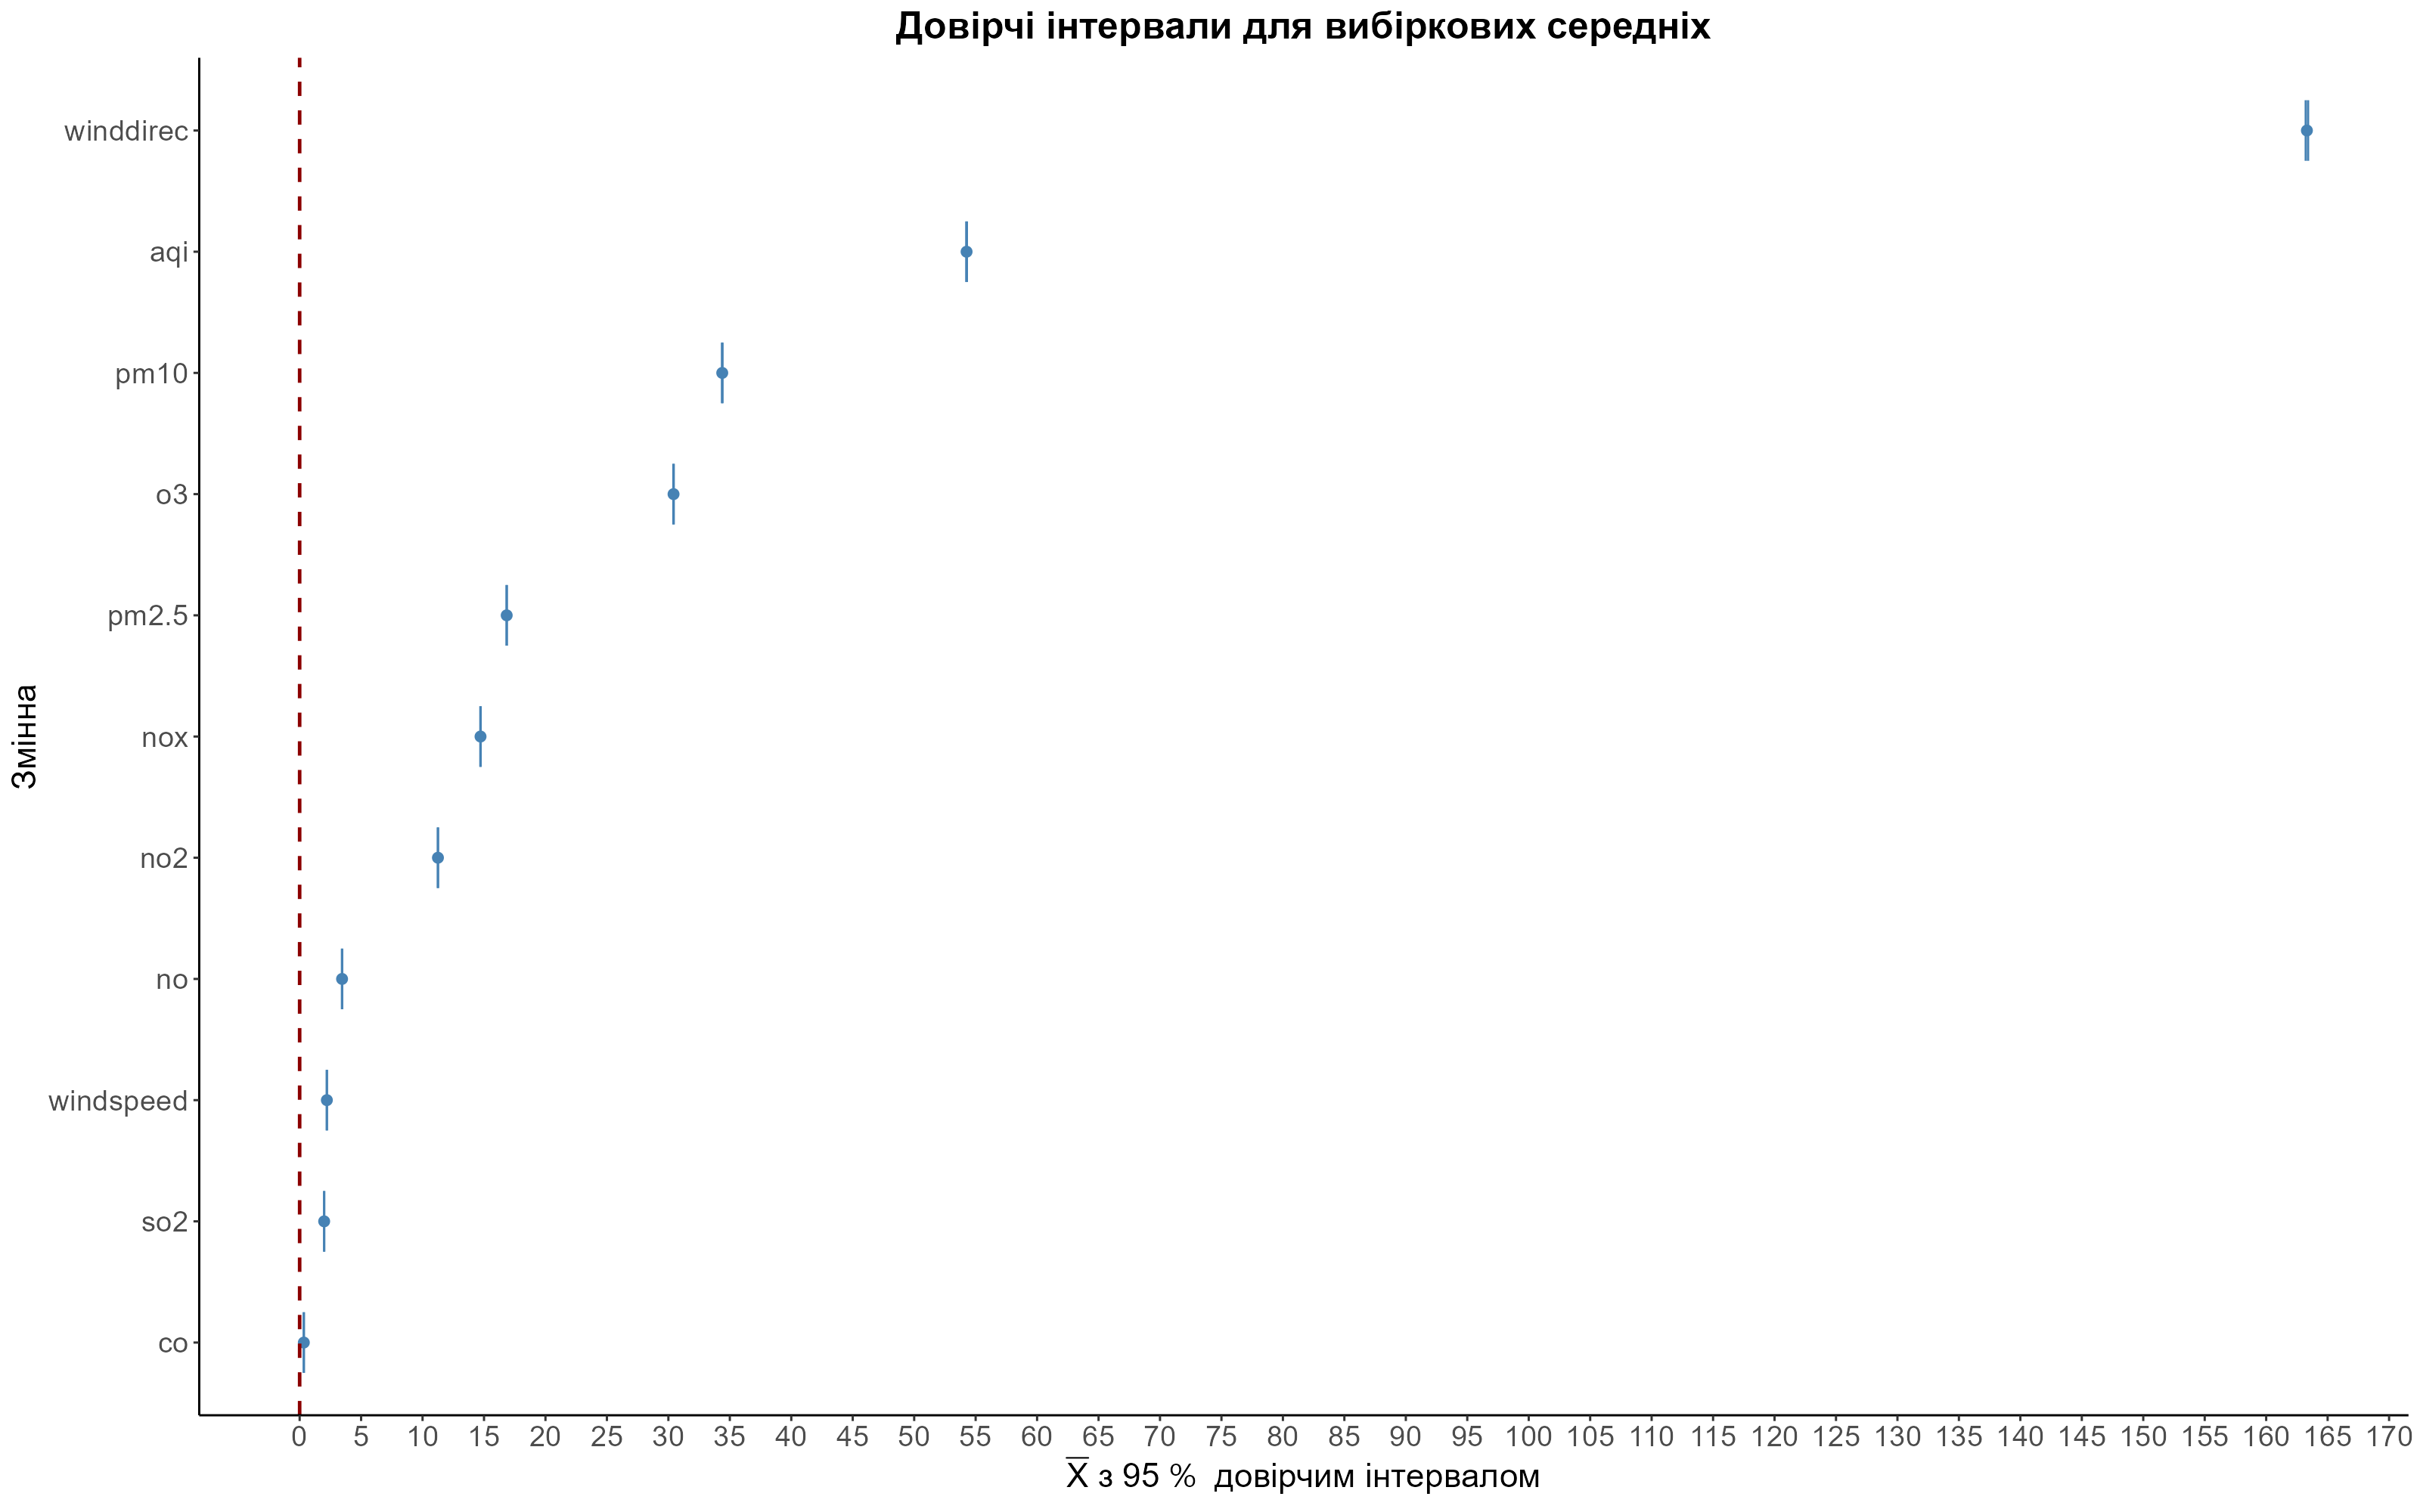
\includegraphics[width=\linewidth]{./plots/lab2/1-4-part/ci-means.png}
  \end{center}
  
\end{frame}

\begin{frame}
  \frametitle{Вибіркова дисперсiя}

  Довірчі інтервали для вибіркової дисперсiї:

  \begin{table}[ht]
    \centering
    \begin{tabular}{lrrr}
      \hline
      variable  & lower & variance & upper \\ 
      \hline
      aqi       & 887.78 & 888.80 & 889.82 \\ 
      so2       & 2.99 & 3.00 & 3.00 \\ 
      co        & 0.06 & 0.06 & 0.06 \\ 
      o3        & 336.27 & 336.66 & 337.06 \\ 
      pm10      & 589.18 & 589.86 & 590.55 \\ 
      pm2.5     & 161.06 & 161.25 & 161.44 \\ 
      no2       & 75.24 & 75.32 & 75.41 \\ 
      nox       & 221.24 & 221.50 & 221.76 \\ 
      no        & 69.76 & 69.85 & 69.93 \\ 
      windspeed & 2.87 & 2.87 & 2.87 \\ 
      winddirec & 13104.48 & 13119.86 & 13135.27 \\ 
       \hline
    \end{tabular}
  \end{table}
\end{frame}

\begin{frame}
  \frametitle{Вибіркова дисперсiя}

  \begin{center}
    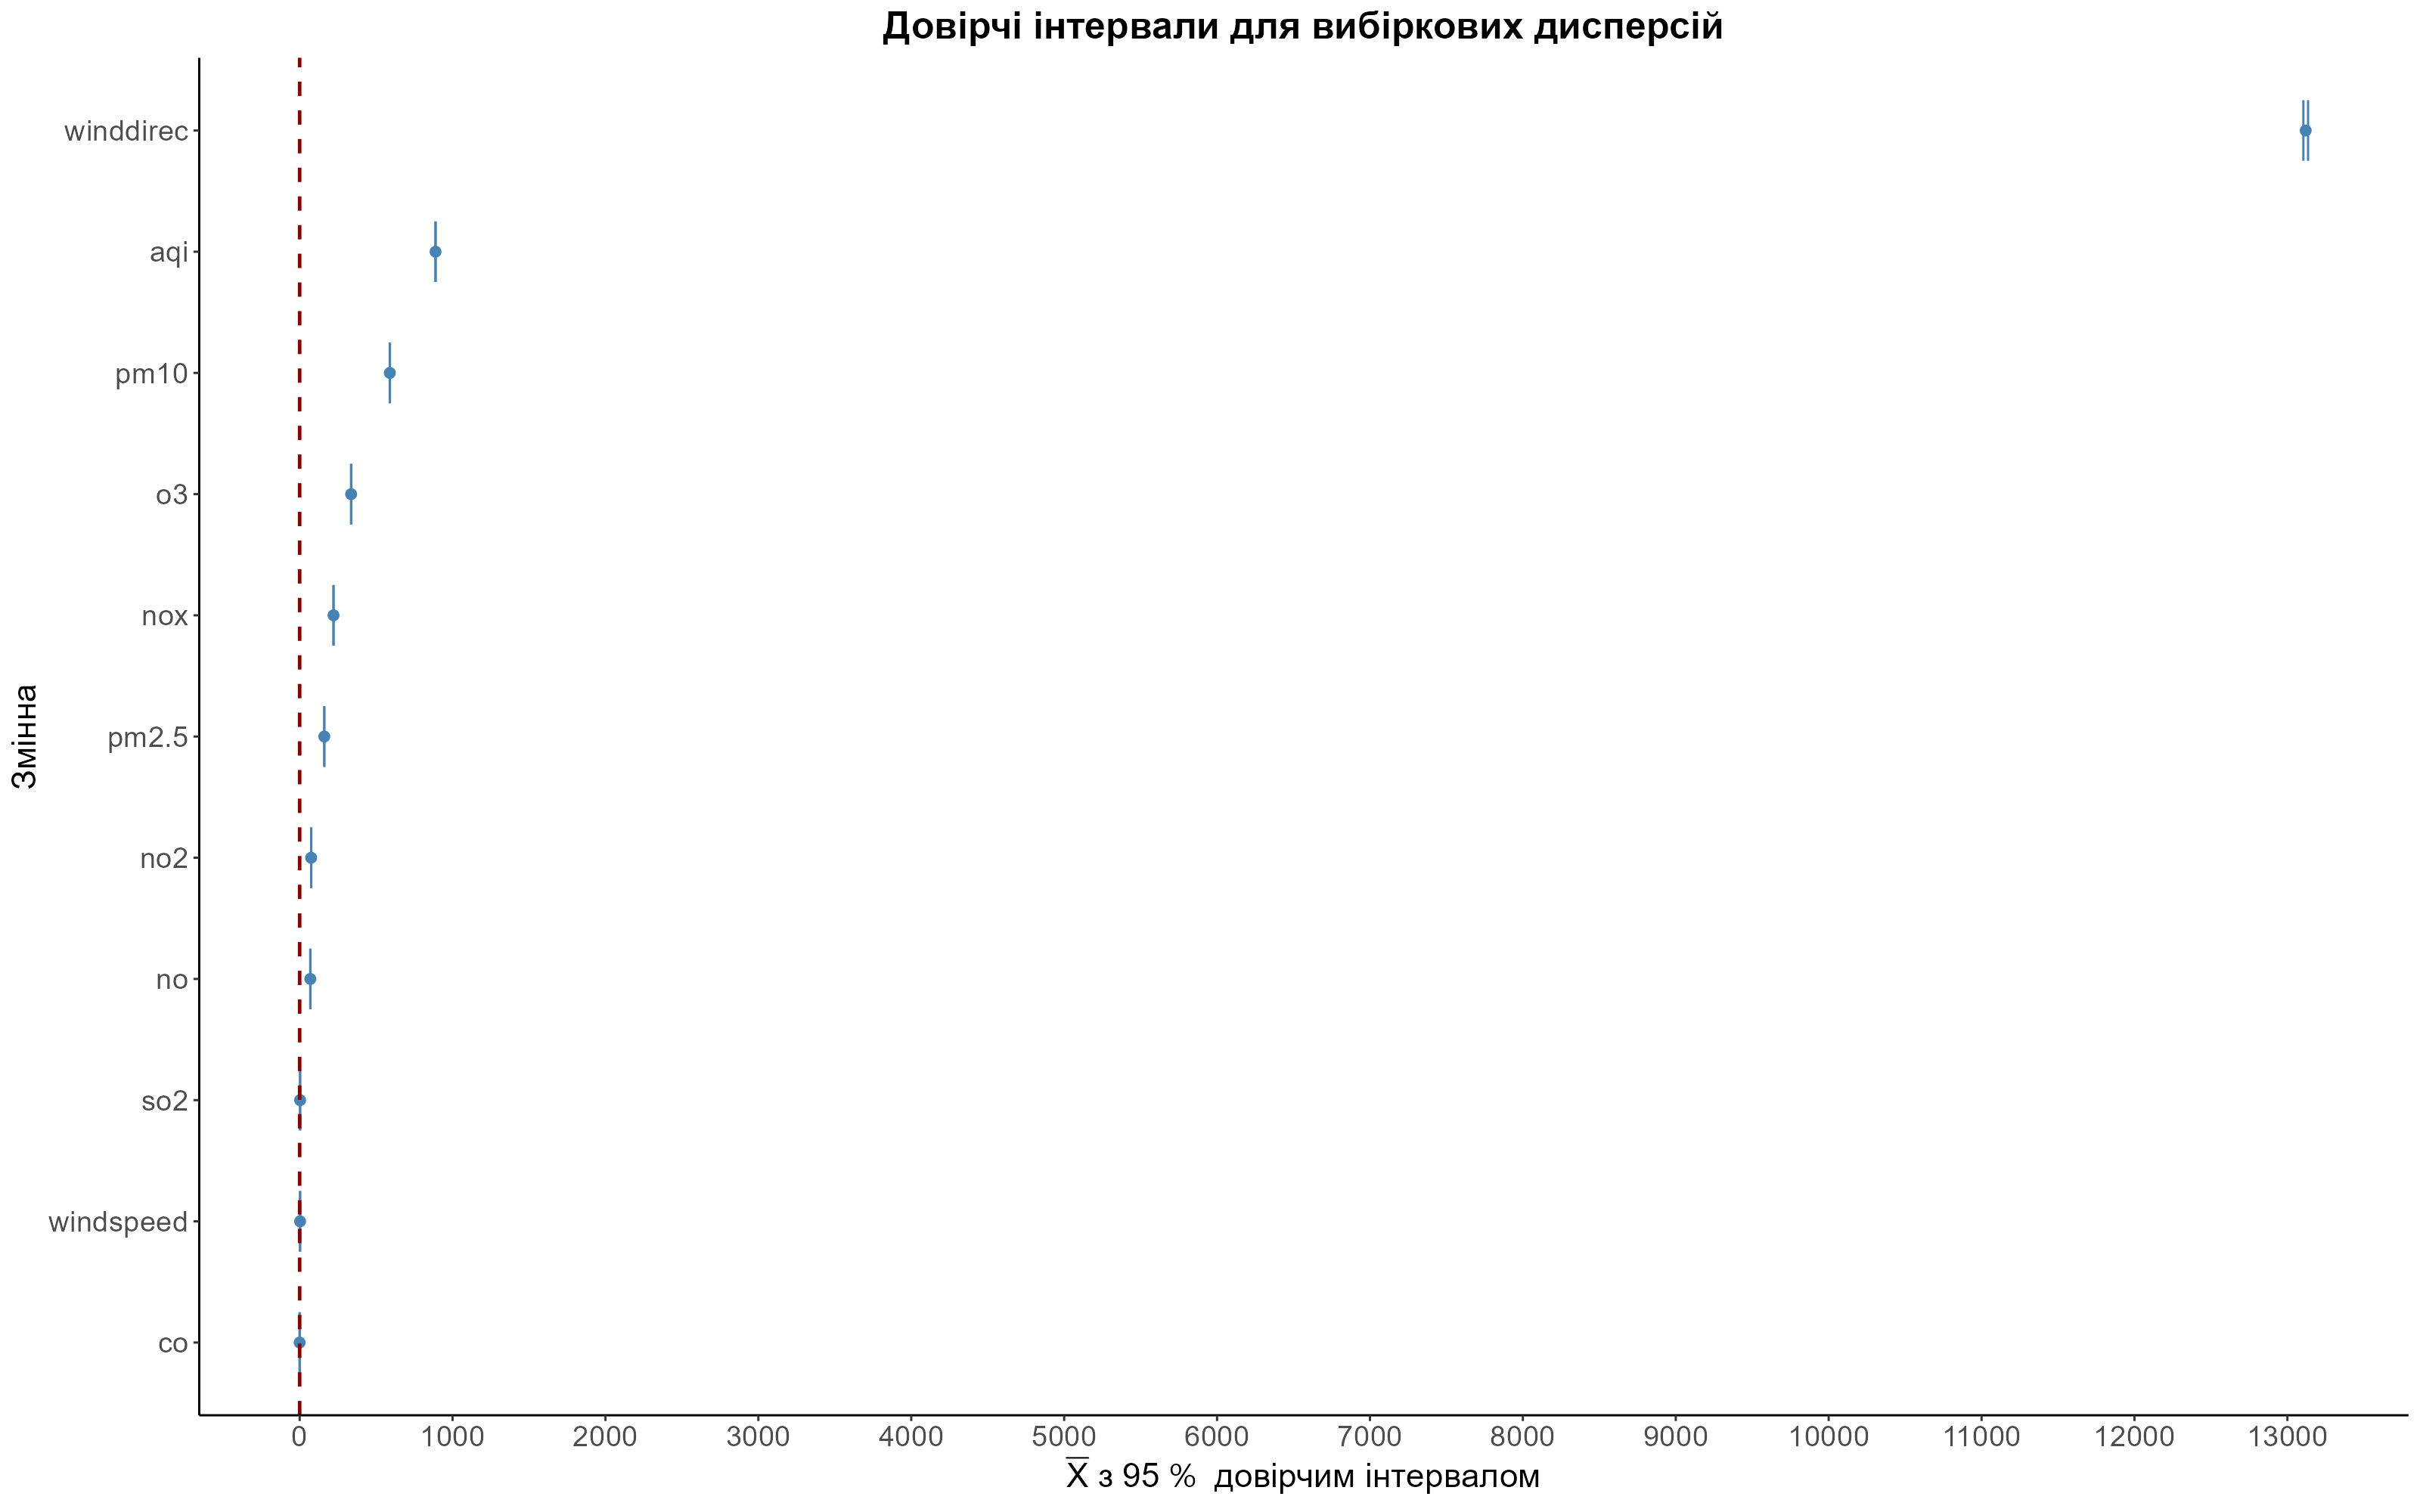
\includegraphics[width=\linewidth]{./plots/lab2/1-4-part/ci-var.png}
  \end{center}
  
\end{frame}

\begin{frame}[fragile=singleslide]
  \frametitle{Висновки}

  \begin{enumerate}
    \item Змінні, такі як $winddirec$ і $AQI$, мають відносно широкі 
    довірчі інтервали для середніх та дисперсії, що свідчить про високу
    невизначеність
    \item $SO_2$, $CO$ та інші мають вузькі інтервали, що вказує на
    більш стабільні або точні вимірювання.
  
  \end{enumerate}
\end{frame}

\begin{frame}
  \frametitle{AQI по регіонам}

  Розглянемо AQI по регіонам і розділимо їх на рік до реформи та рік після.

  \begin{itemize}
    \item Розглянемо 16 та 17 роки 
    \item Розглянемо 23 та 24 роки 
  \end{itemize}
\end{frame}

\begin{frame}
  \frametitle{AQI по регіонам}

  \begin{center}
    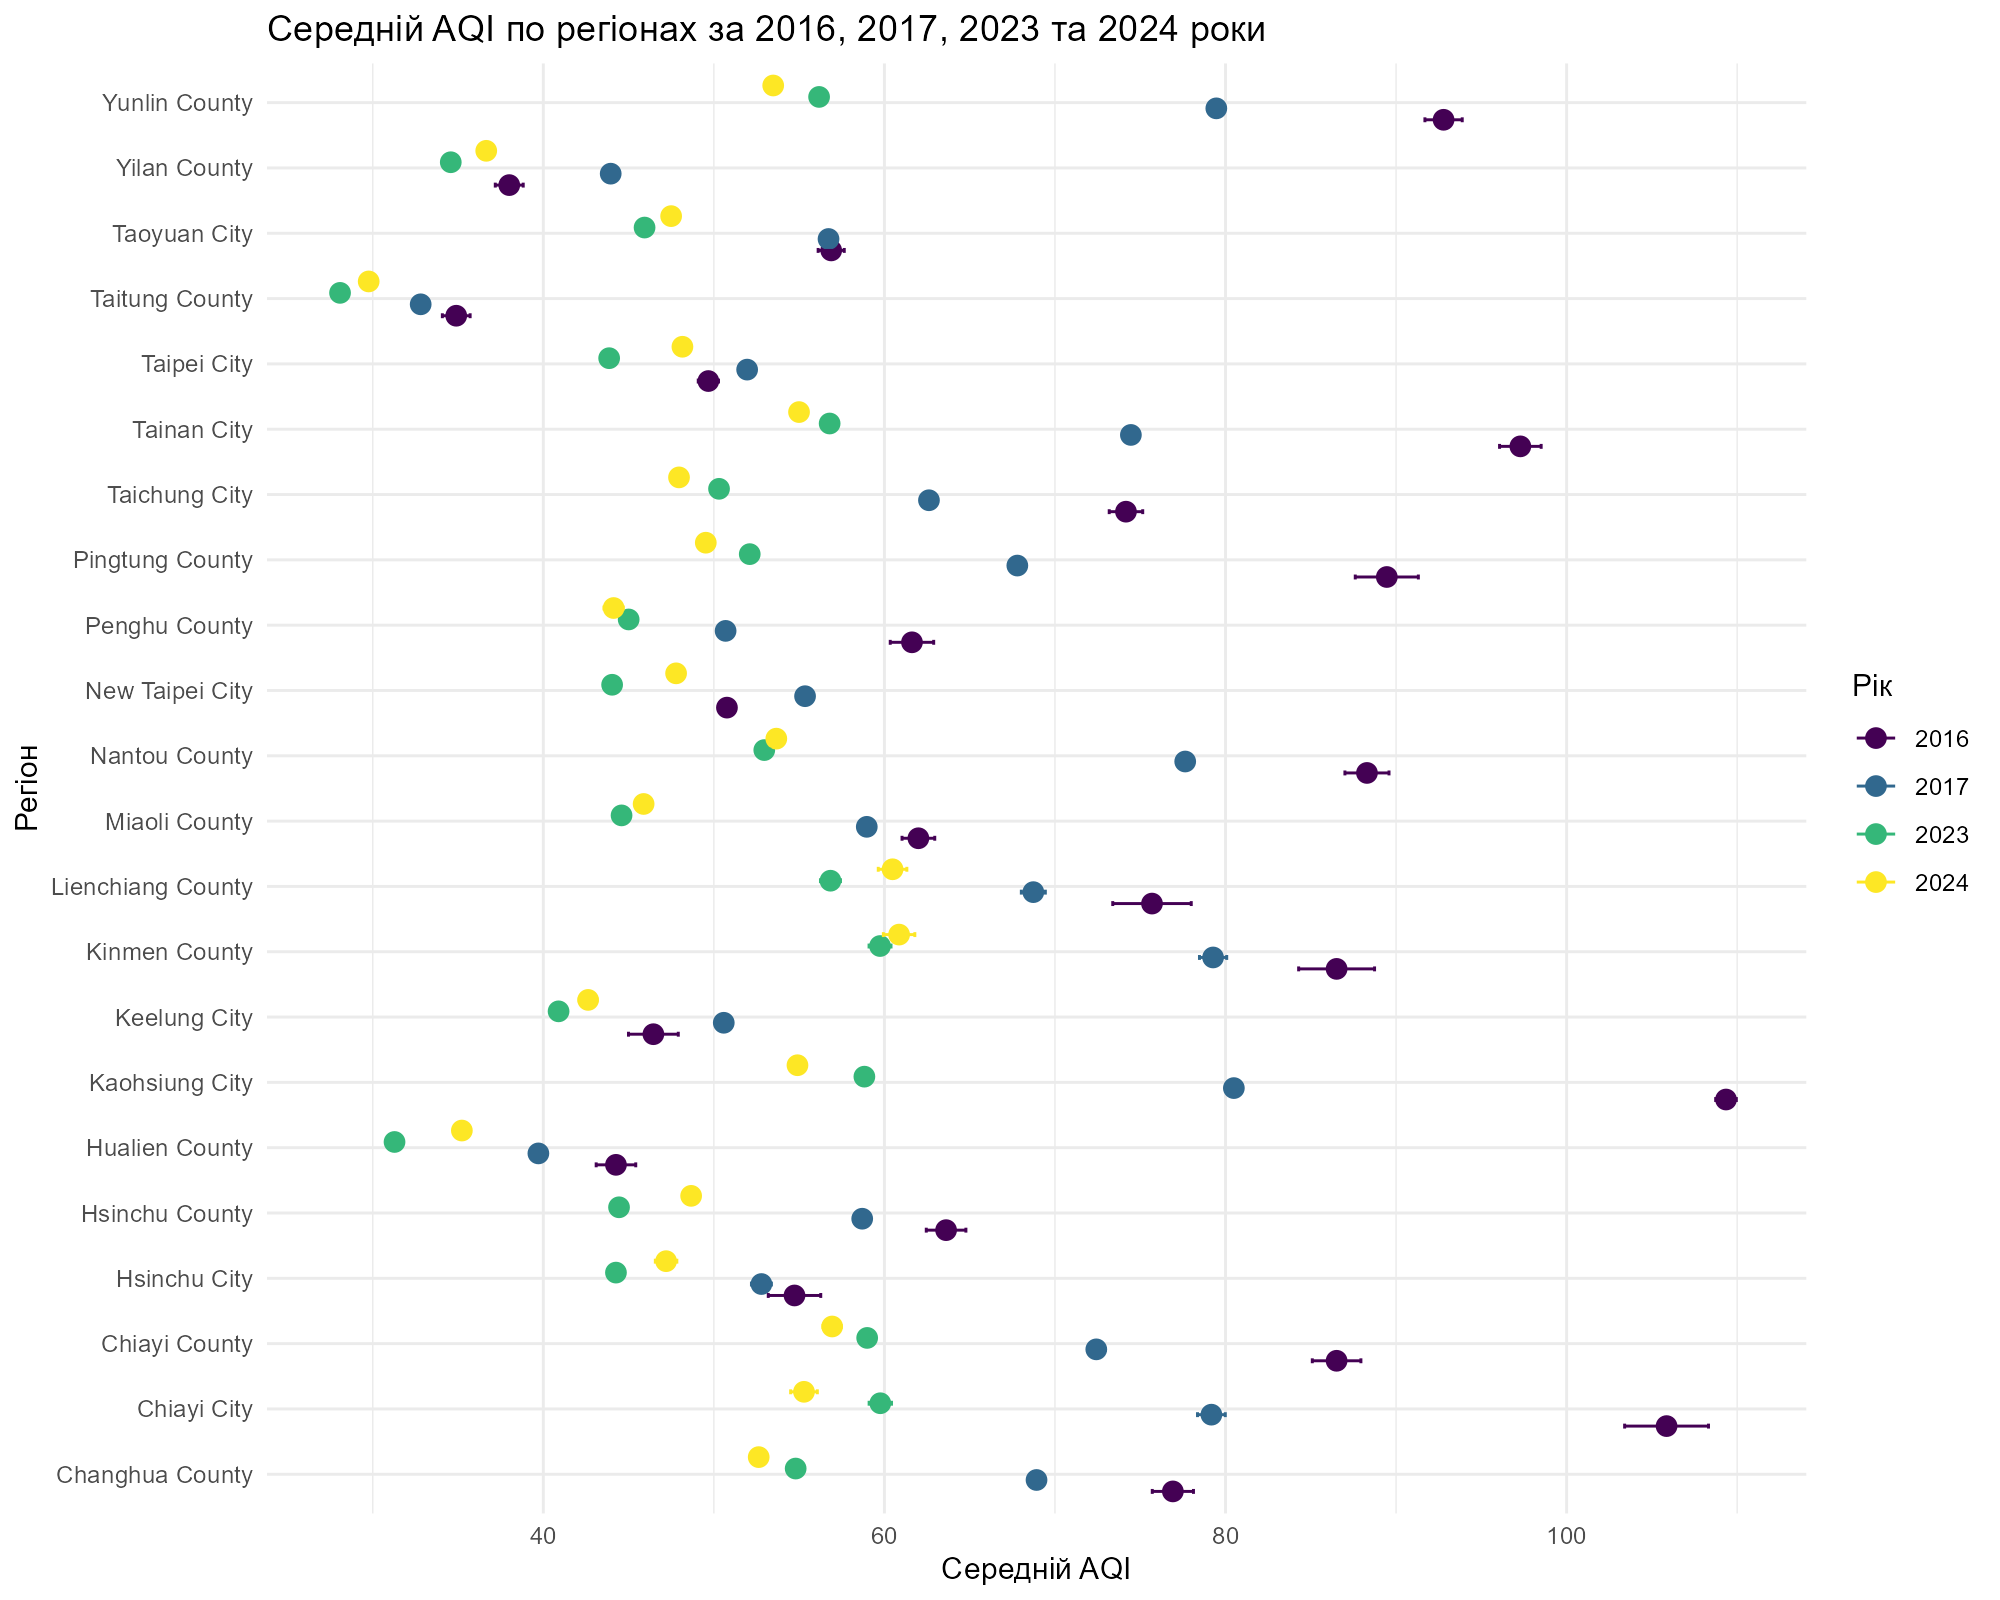
\includegraphics[height=3in]{./plots/lab2/1-4-part/aqi_by_year_region.png}
  \end{center}
\end{frame}

\begin{frame}
  \frametitle{Висновки}

  \begin{enumerate}
    \item Загально бачимо позитивні зміни. 
    Збільшується кількість вимірювань в кожному регіоні з кожним роком. 
    Середні показники зменшуються.
    \item Розгленемо AQI по регіонам до та після реформи.
  \end{enumerate}

  
\end{frame}

\begin{frame}
  \frametitle{AQI по регіонам до та після реформи}

  \begin{center}
    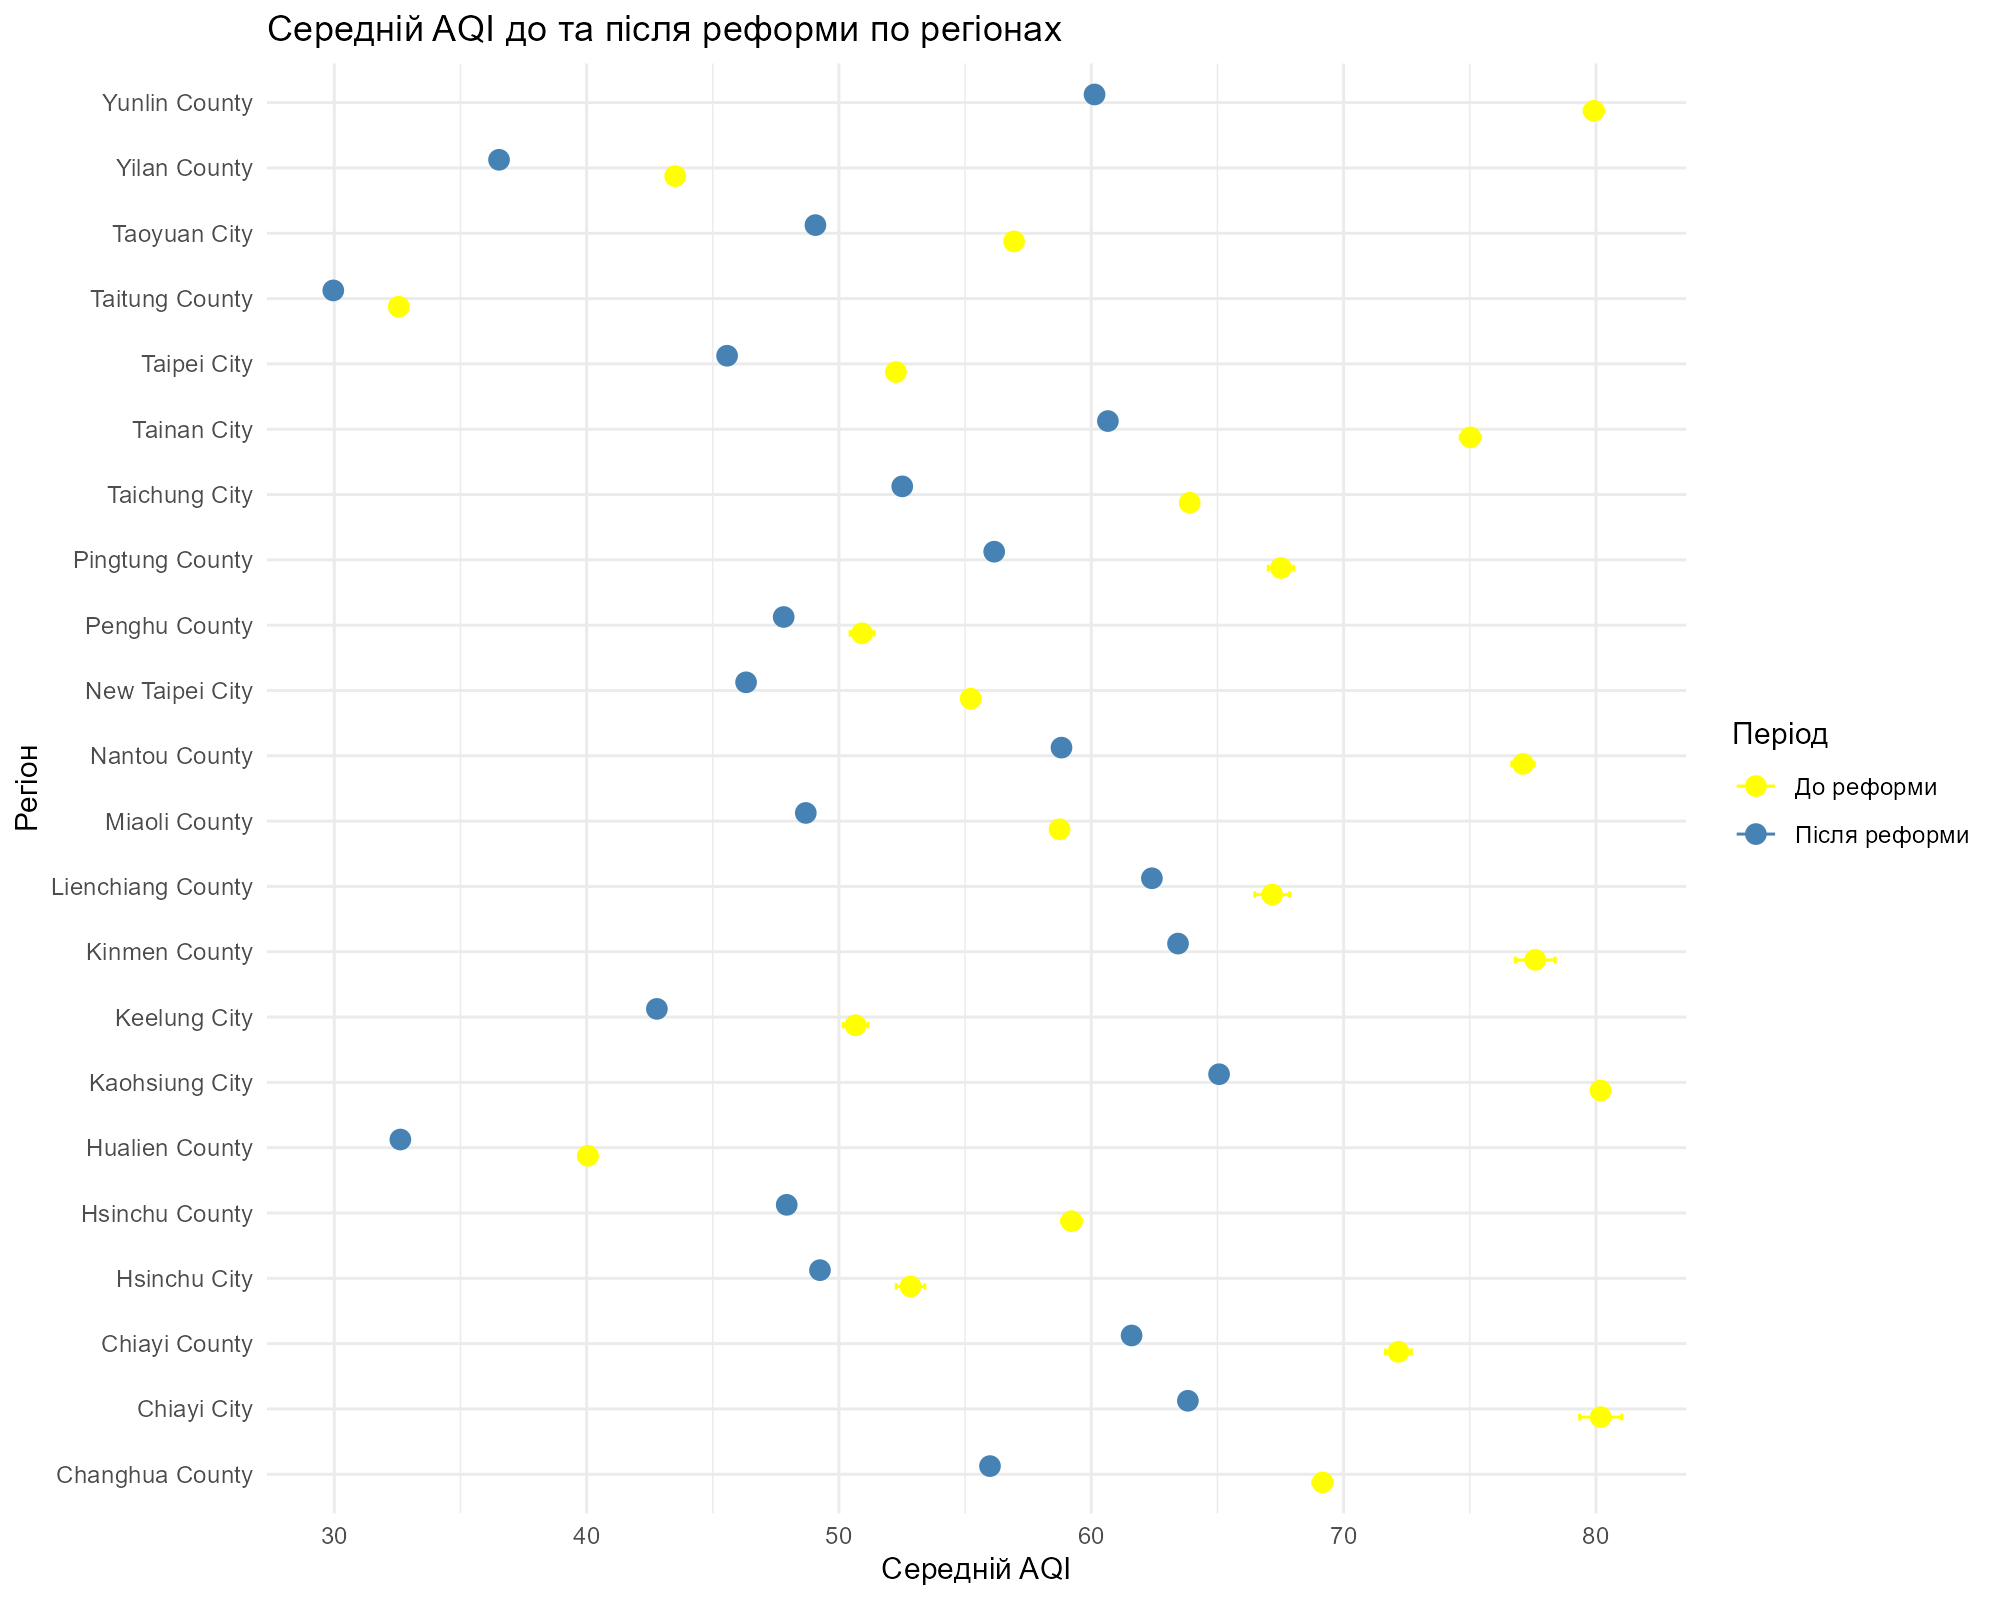
\includegraphics[height=3in]{./plots/lab2/1-4-part/aqi_comparison_before_after.png}
  \end{center}

\end{frame}

\begin{frame}
  \frametitle{Висновки}

  % TODO: Тут мав би бути висновок до попереднього слайду

\end{frame}


\begin{frame}
  \frametitle{Перша група}

  \begin{center}
    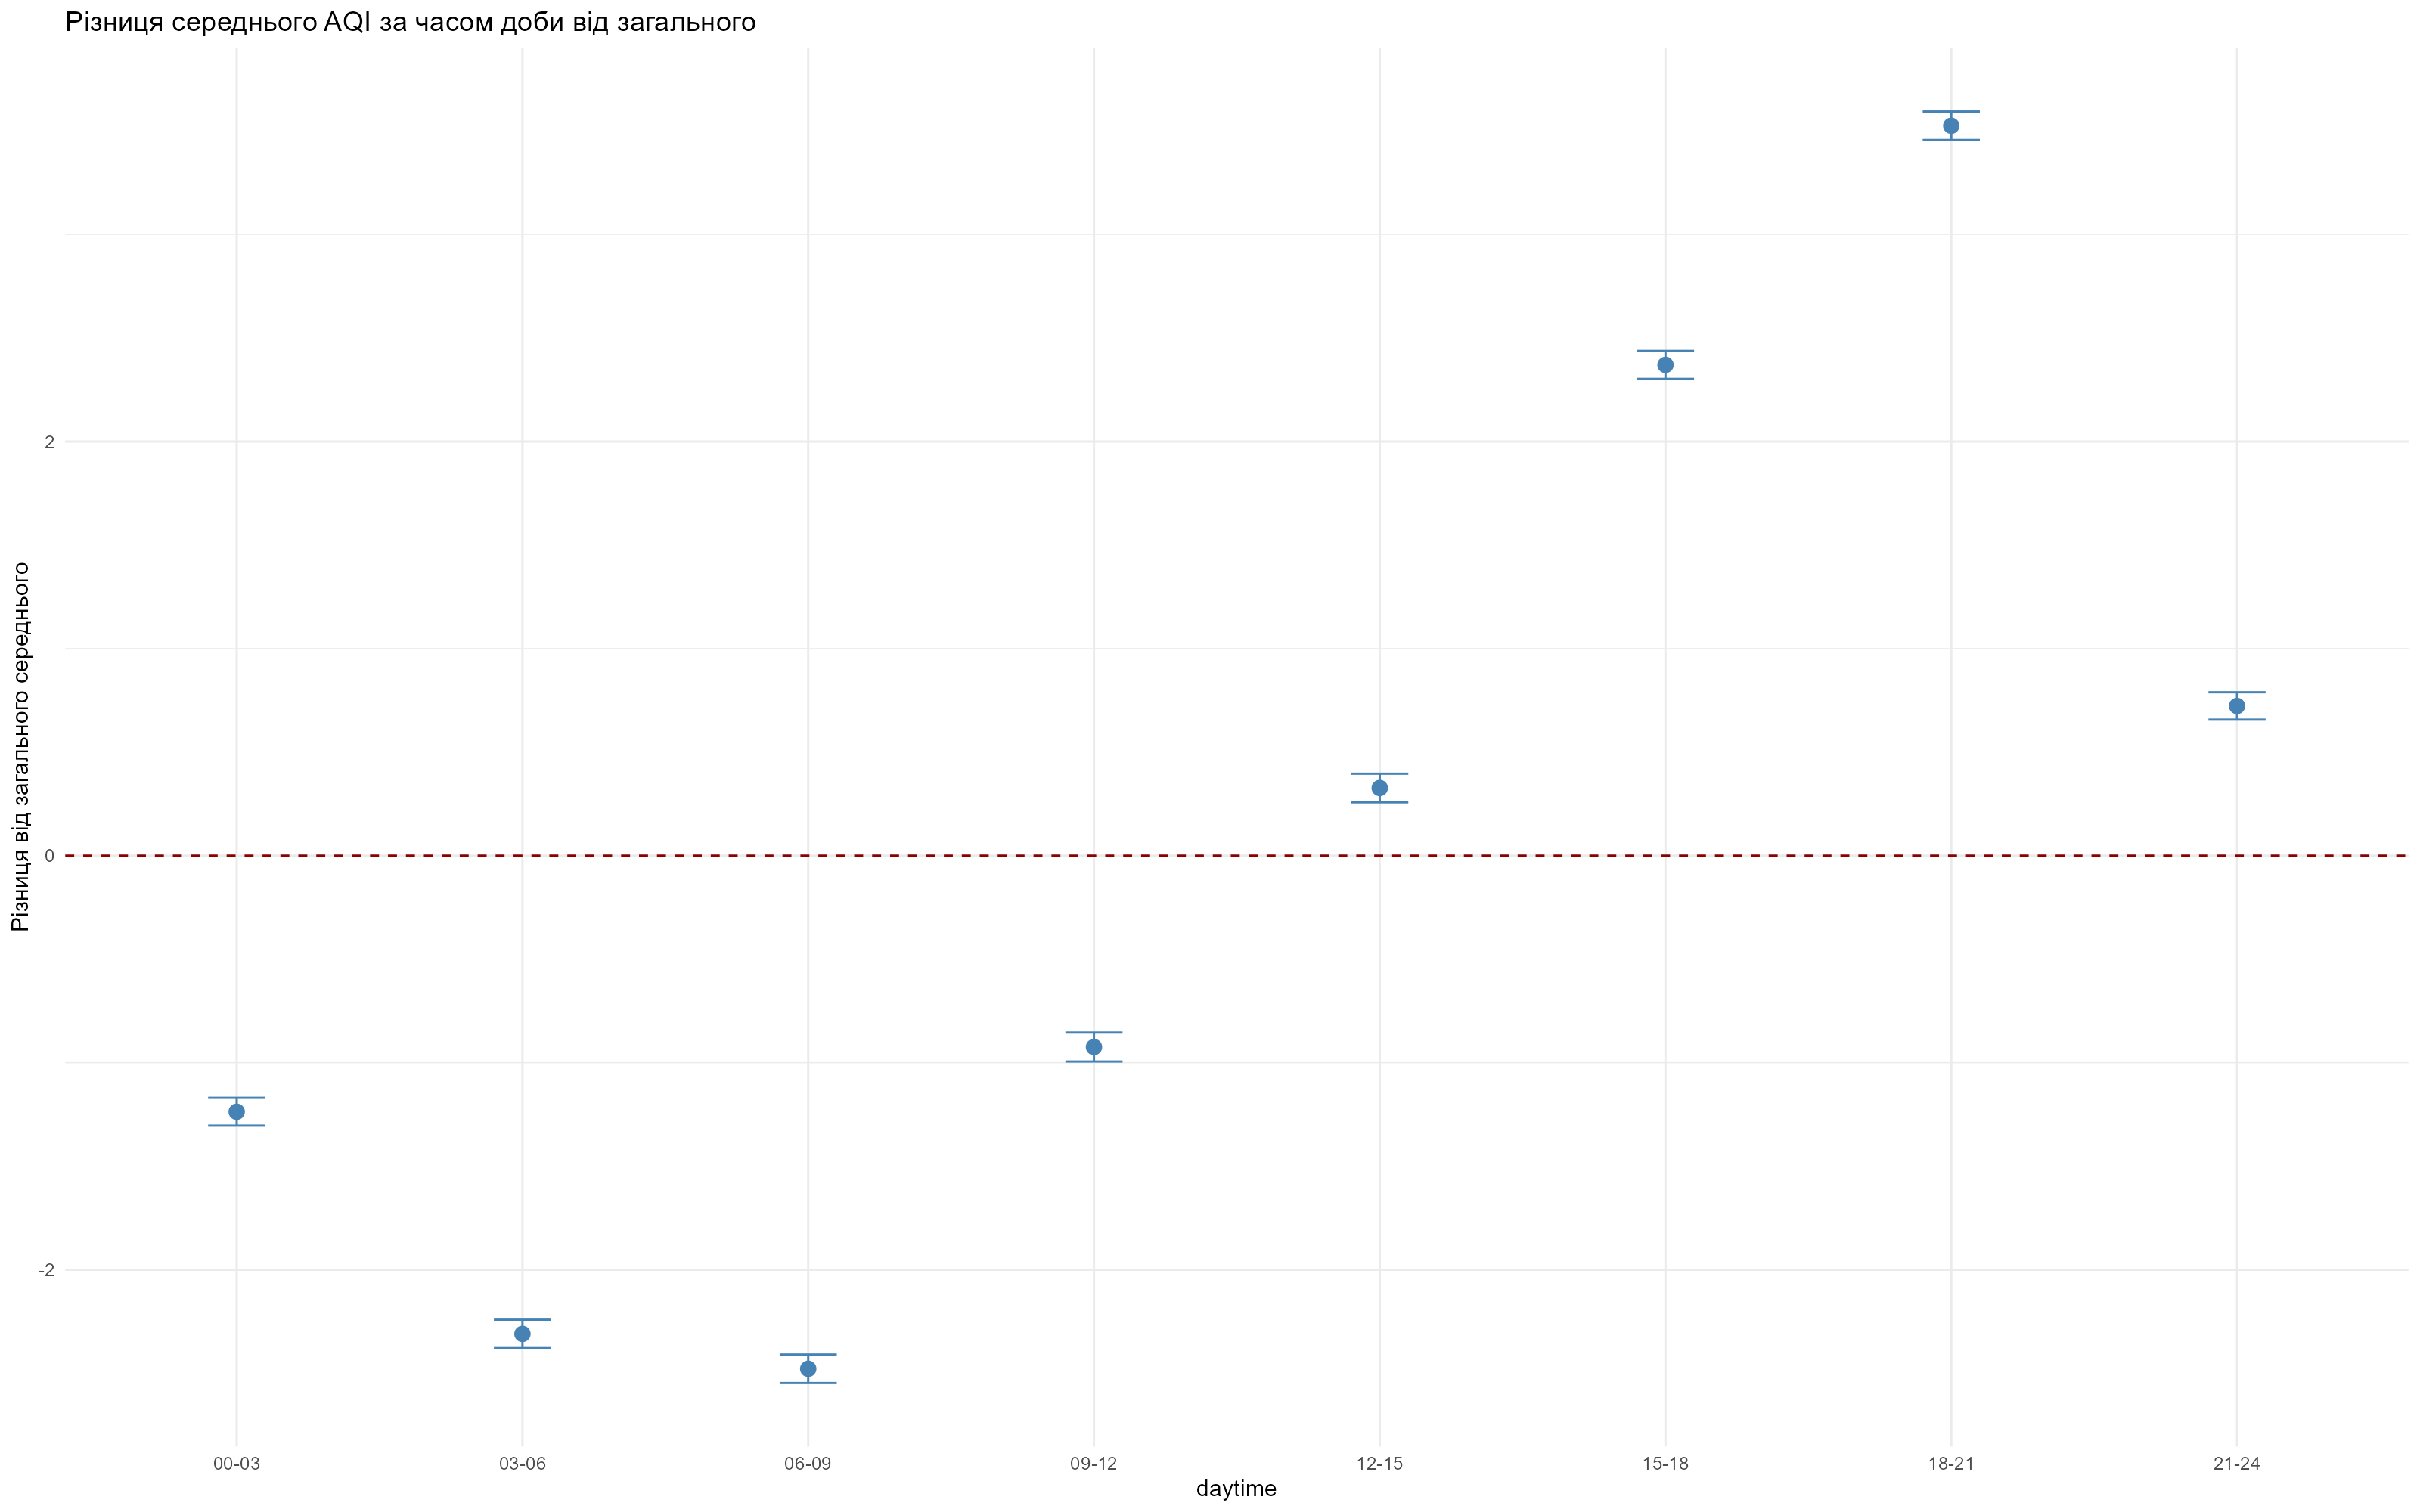
\includegraphics[height=2.7in]{./plots/lab2/1-4-part/daytime_summary.png}
  \end{center}

\end{frame}

\begin{frame}
  \frametitle{Перша група}

  \begin{enumerate}
    \item Бачимо, що AQI впродовж доби має різні значення.
    \item Найвищі значення AQI спостерігаються в період з 12 до 15 години, 
    що може бути пов'язано з підвищеною активністю транспорту та промисловості в цей час.
  
  \end{enumerate}
\end{frame}

\begin{frame}
  \frametitle{Перша група}

  \begin{center}
    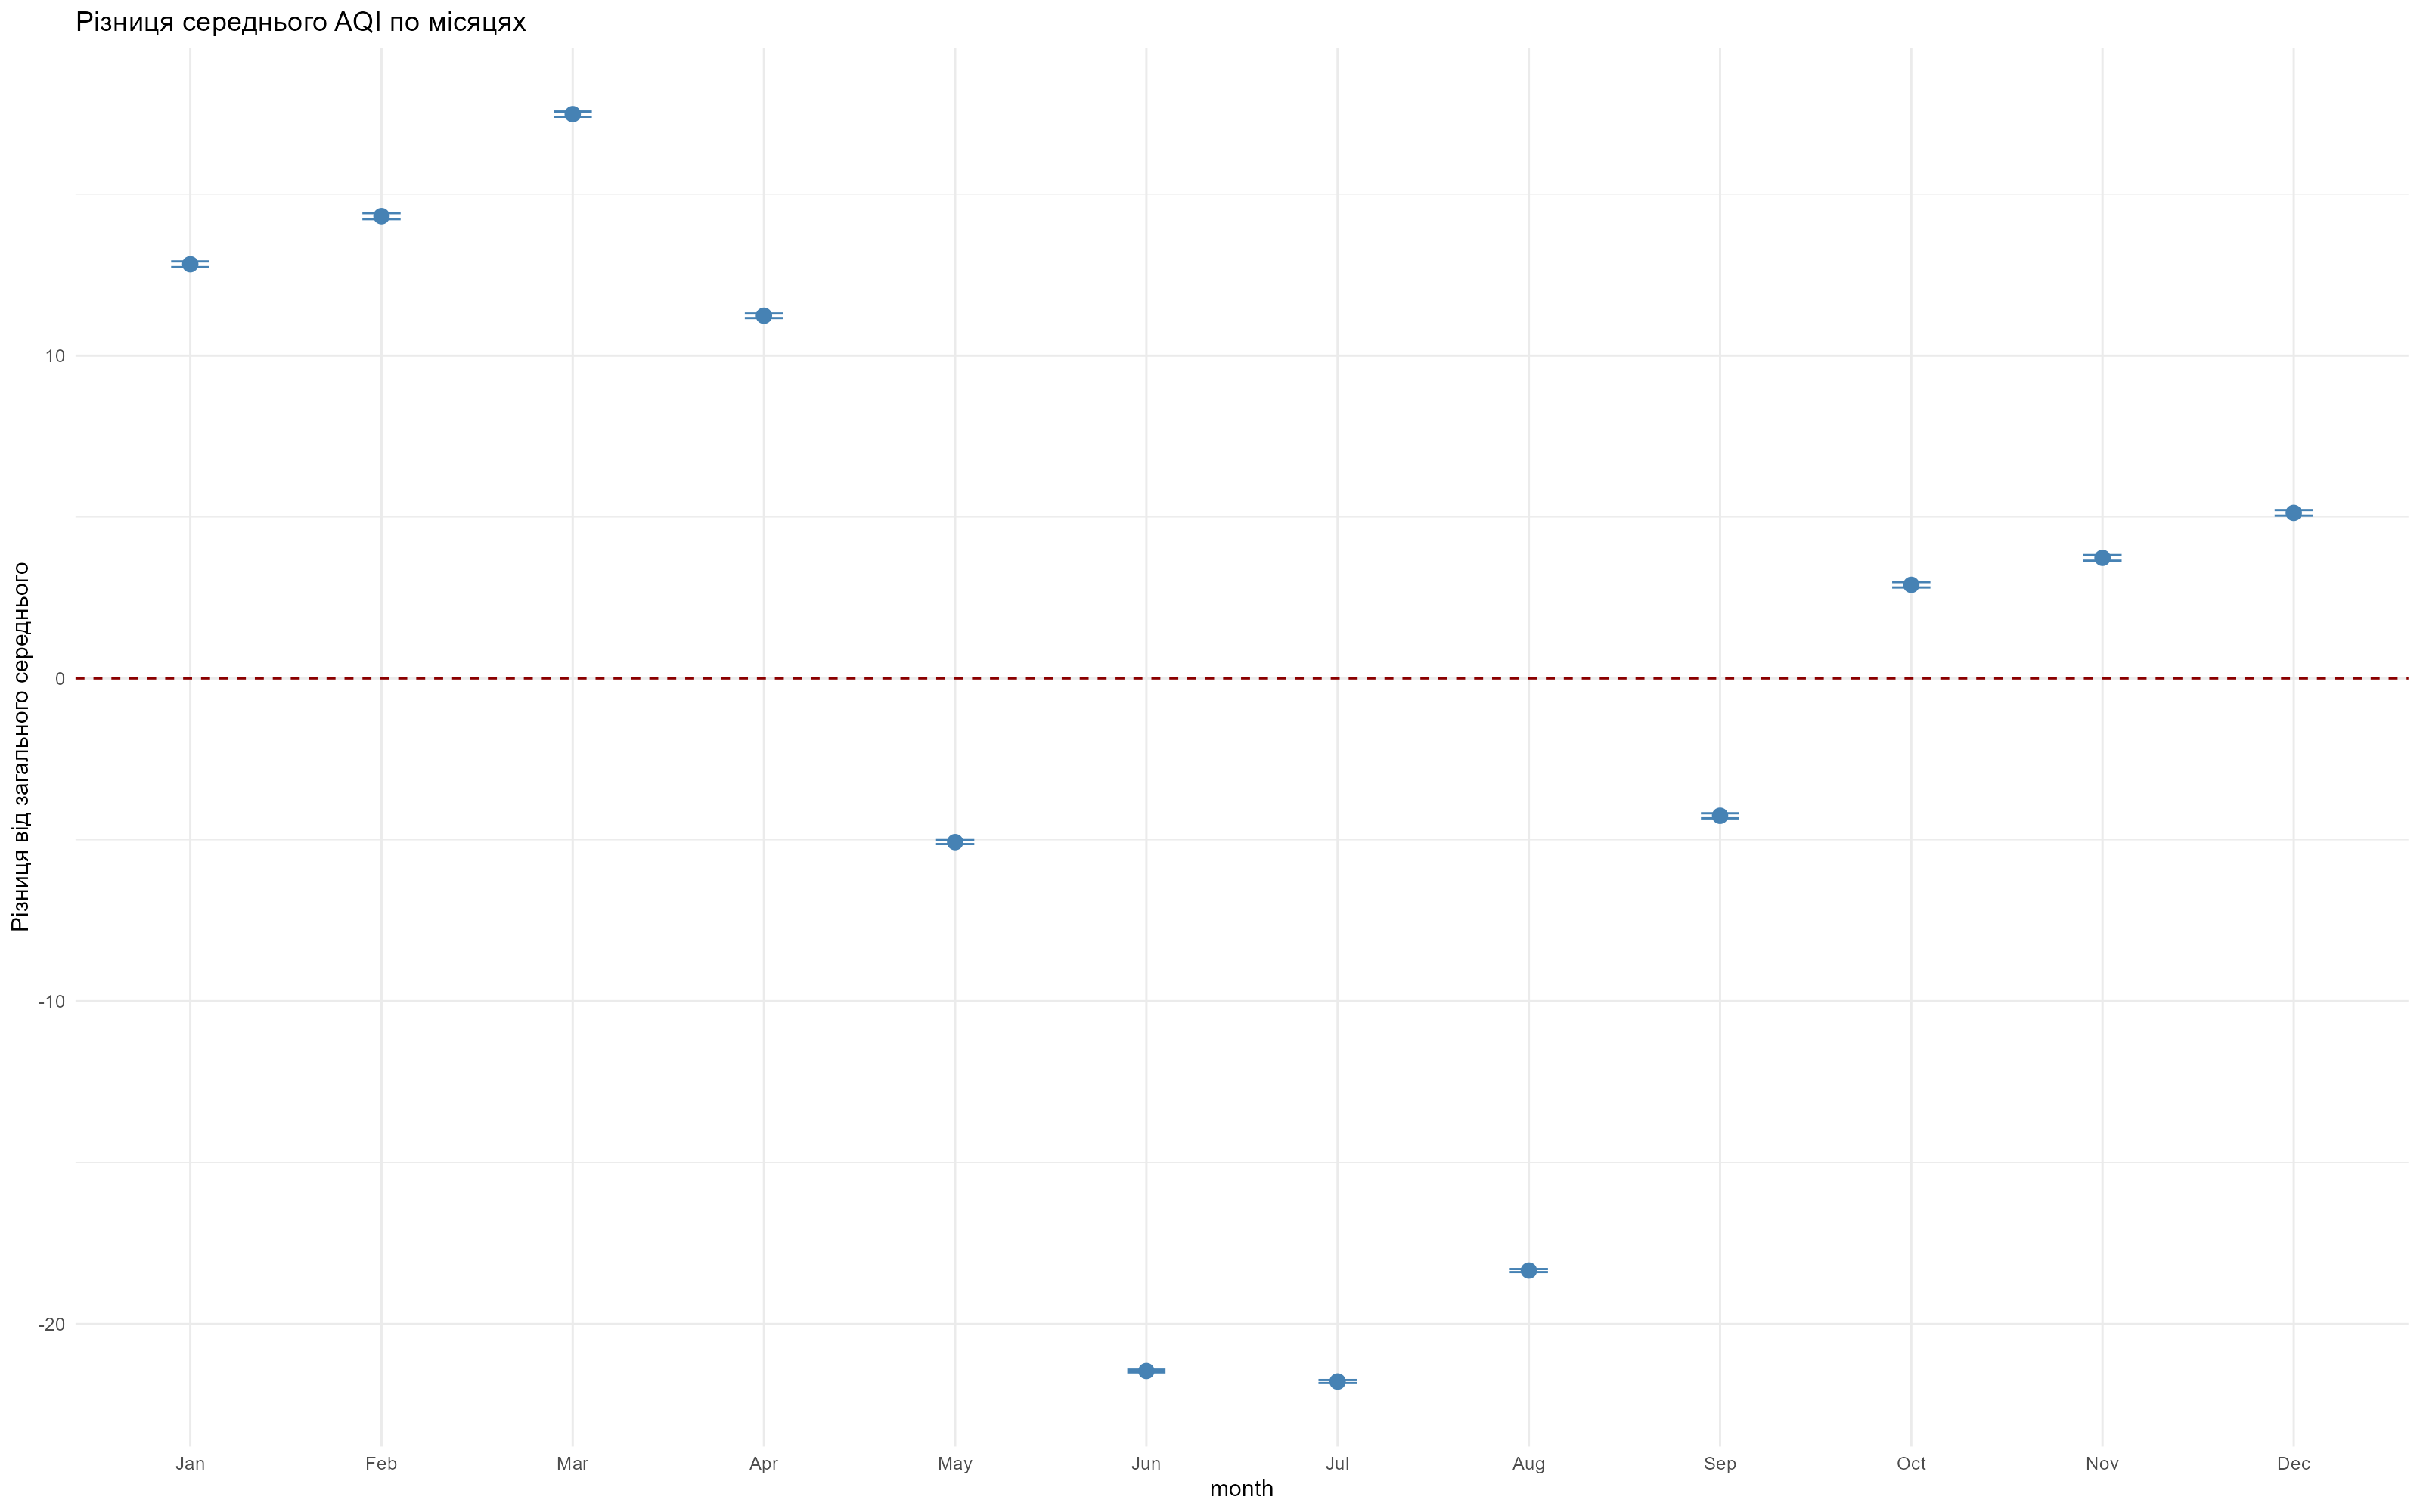
\includegraphics[height=2.7in]{./plots/lab2/1-4-part/seasonal_summary.png}
  \end{center}

\end{frame}

\begin{frame}
  \frametitle{Перша група}

  \begin{enumerate}
    \item  Бачимо, що AQI впродовж року має різні значення.
    \item Найвищі значення AQI спостерігаються в червні та липні, 
    що може бути пов'язано з підвищеною температурою повітря та забрудненням від 
    літніх активностей.
  
  \end{enumerate}
\end{frame}

% TODO: Тут має бути візуалізація для третьої групи

\begin{frame}
  \frametitle{Третя група}

  \begin{enumerate}
    \item Для більшості кореляцій, інтервали не охоплюють нуль, що може свідчити про
    статистичну значущість цих кореляцій. Це в свою чергу може вказувати на те,
    що між змінними є справжня лінійна залежність, а не випадкова.
    \item Інтервали для коефіцієнтів кореляції різняться між методами 
    (Normal, Basic, Percentile, Bca, Student), але загальна картина не сильно 
    змінюється, і всі інтервали підтверджують позитивні або негативні кореляції. 
    
    % TODO: Формулювання/Доречність
    % \item Бутстреп-довірчі інтервали підтверджують наявність статистично 
    % значущого зв’язку між [X] та [Y], оскільки 0 не входить у жоден з інтервалів. 
    % Для пари [X1] та [Y2] інтервал охоплює 0, отже, висновок про залежність непевний.
  
  \end{enumerate}
\end{frame}

% Блок про формулювання/тестування гiпотез, якi доречнi за наслiдком проведеного ранiше розвiдкового аналiзу.

\begin{frame}
  \section{Гіпотези}

  \frametitle{Зміст}
  \tableofcontents[currentsection]
\end{frame}

\begin{frame}
  \frametitle{Зміни AQI впродовж доби}

  Під час виконання лабораторної роботи №1 було помічено,
  що у другій половині дня AQI трохи вище, ніж у першій. 

  \begin{center}
    \begin{tabular}{cc}
      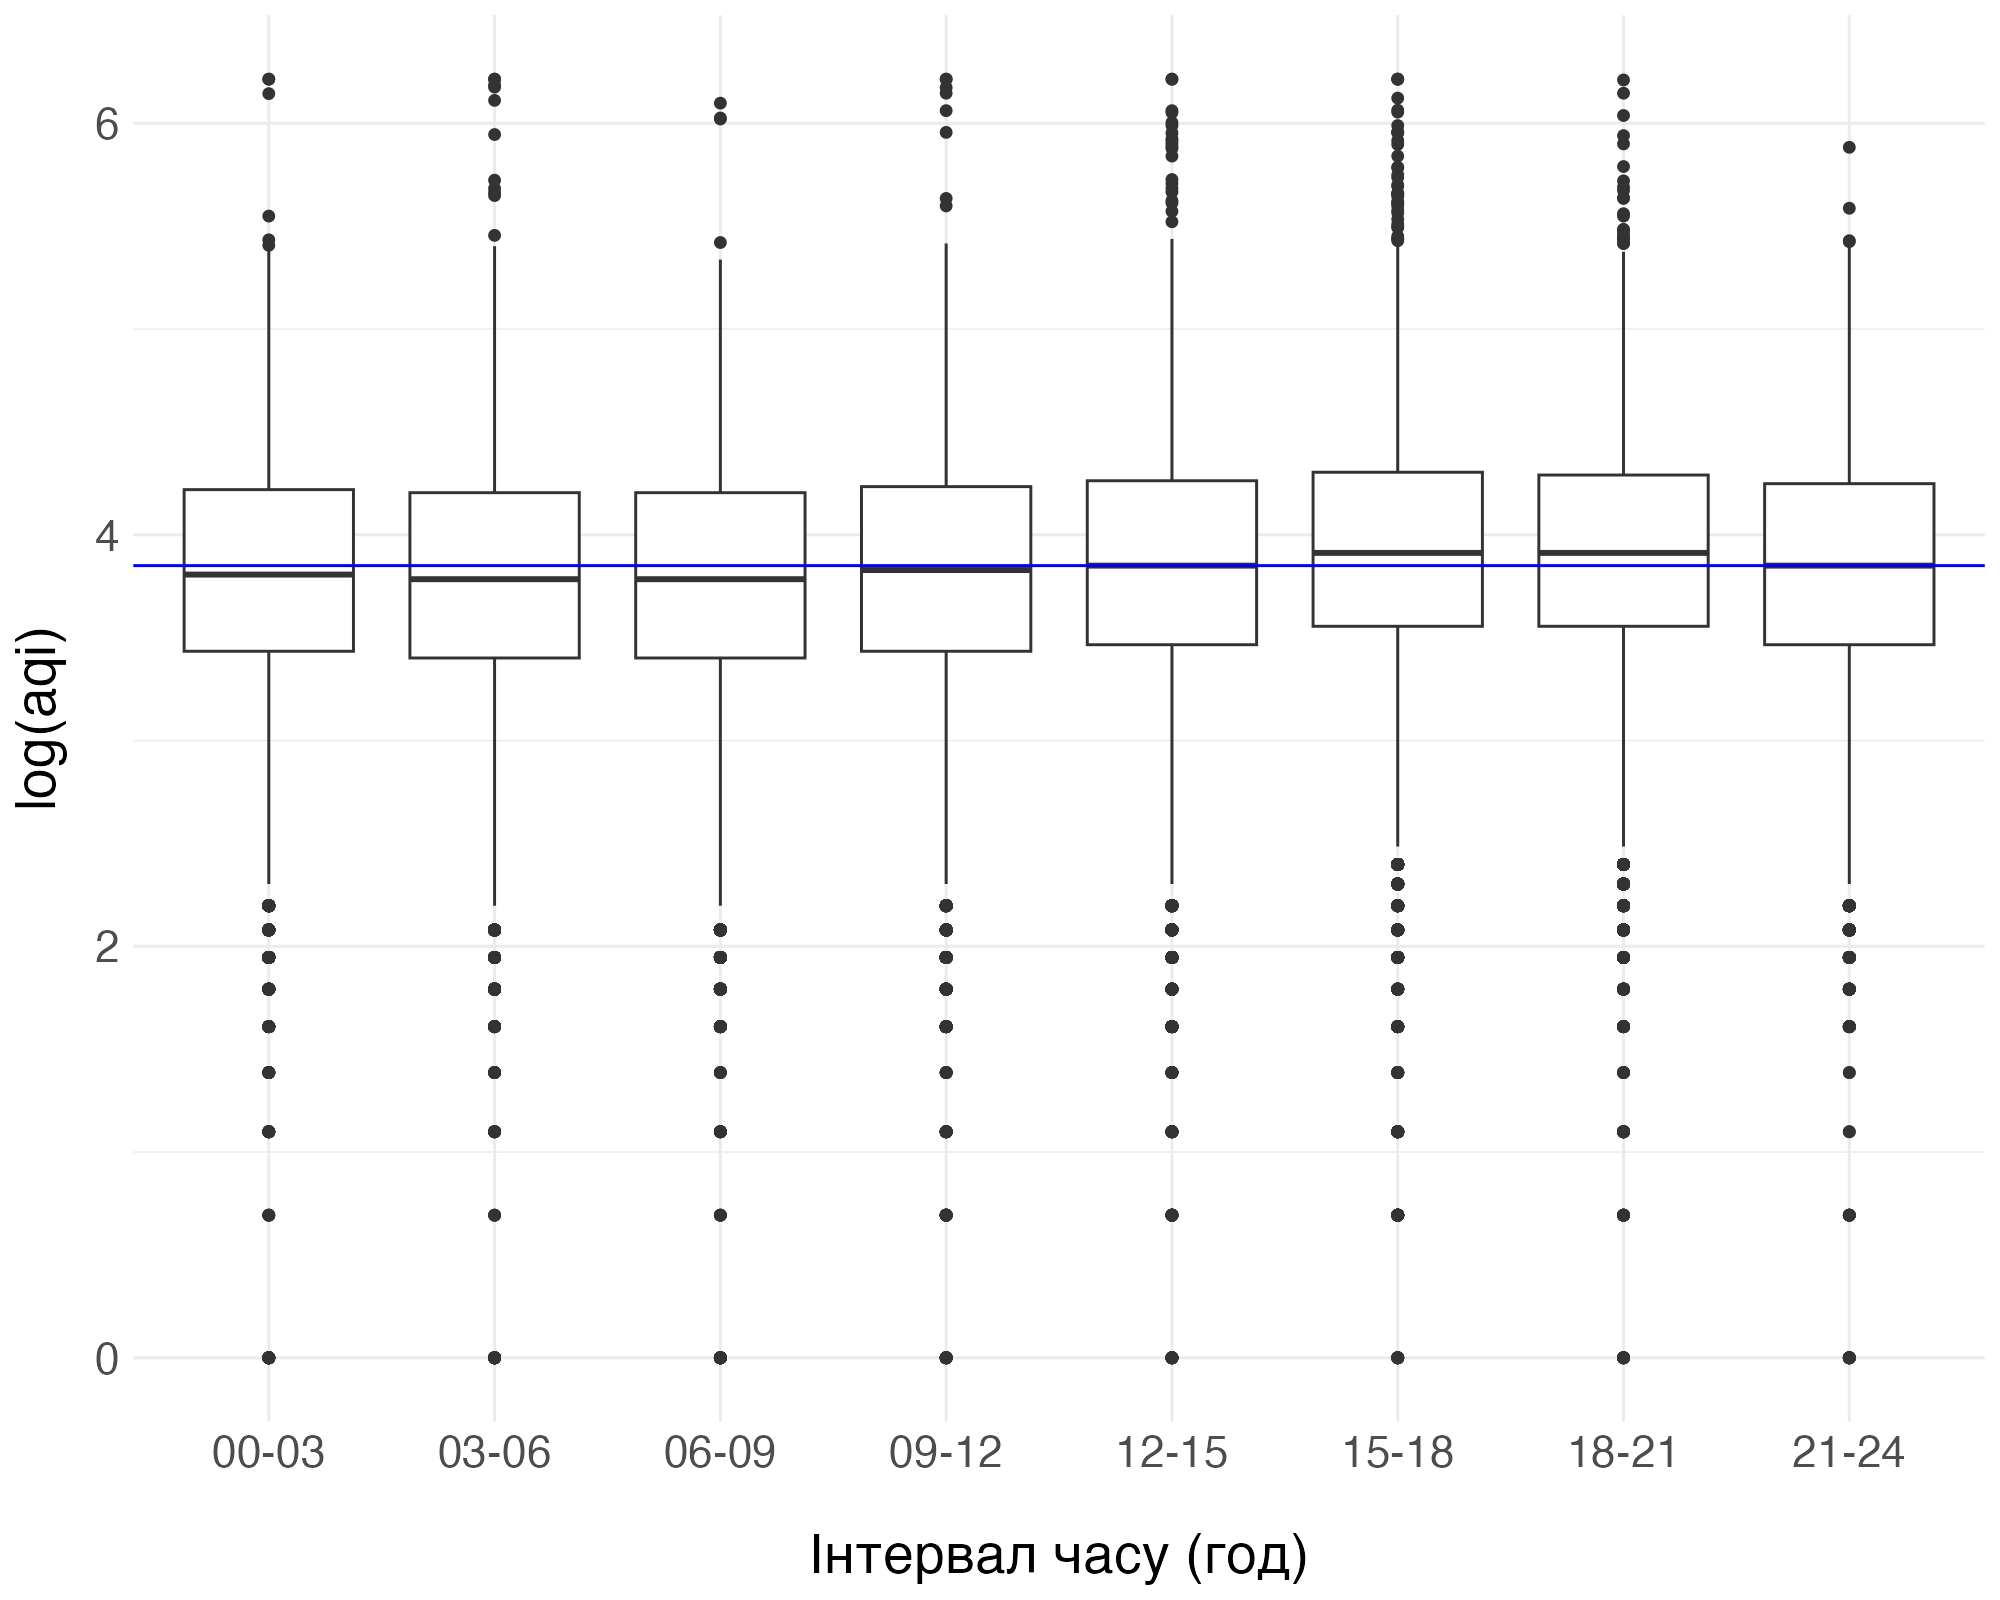
\includegraphics[width=2in]{./plots/lab2/hypotheses/daytime_3hr_vs_aqi.png} &
      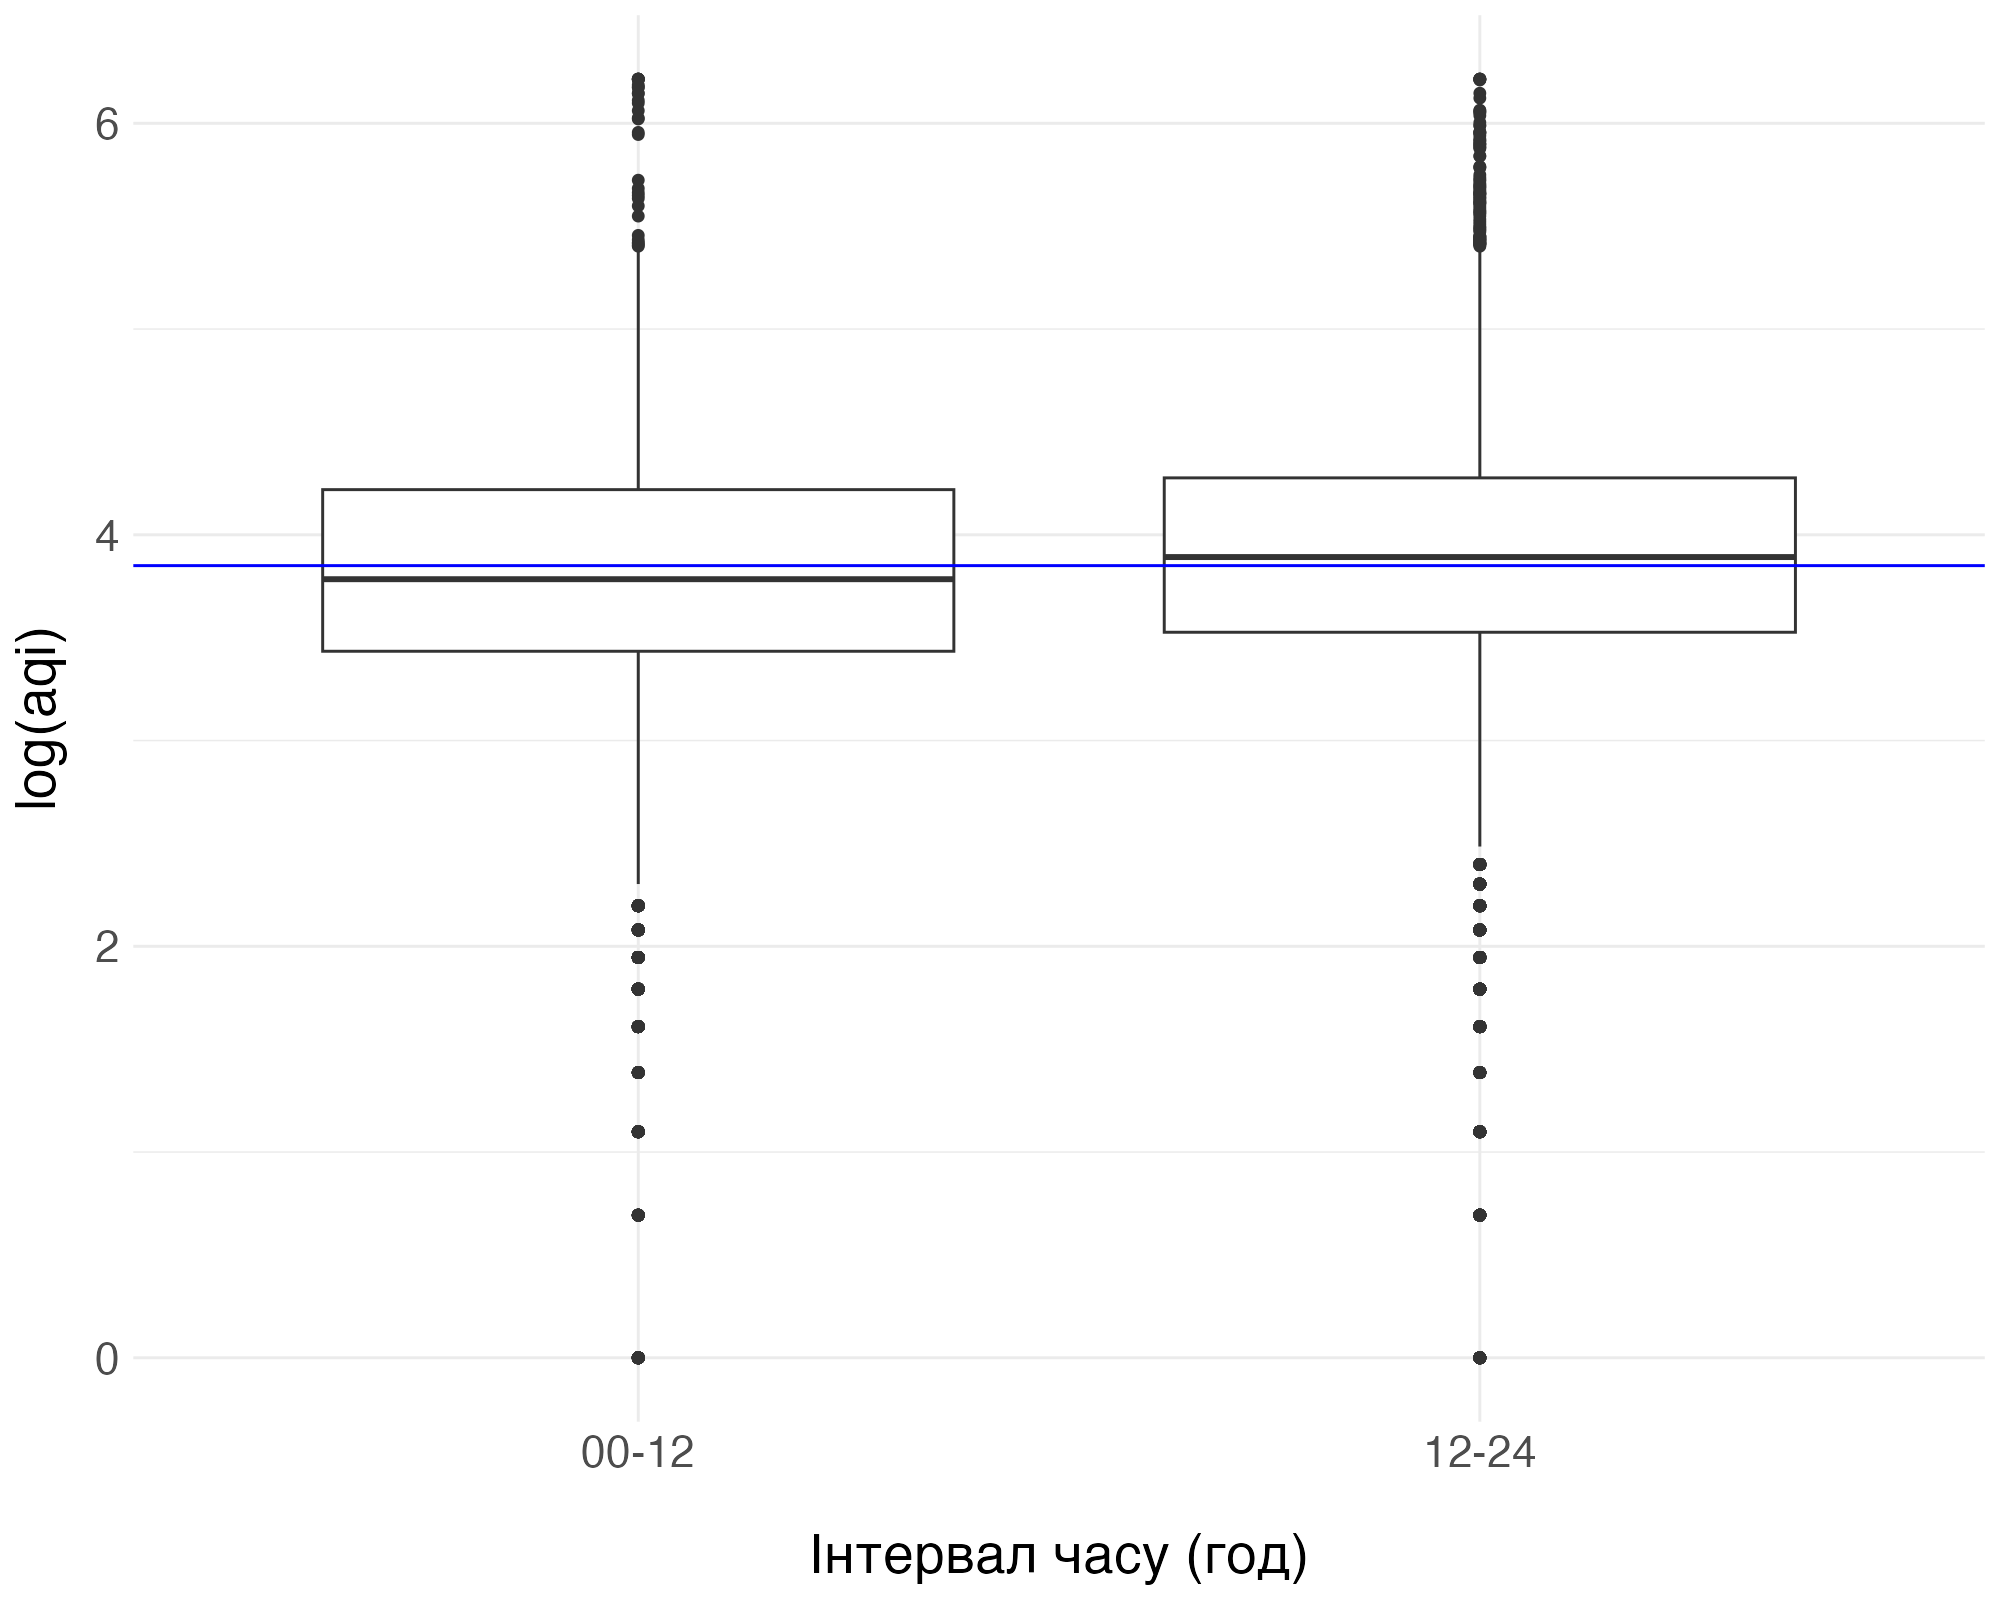
\includegraphics[width=2in]{./plots/lab2/hypotheses/daytime_12hr_vs_aqi.png}
    \end{tabular}
  \end{center}
\end{frame}

\begin{frame}[fragile=singleslide]
  \frametitle{Зміни AQI впродовж доби}

  \begin{enumerate}
    \item Перевіримо, чи є ця різниця статистично значущою.
    \item Розглянемо дві популяції:

      \begin{itemize}
        \item $X$ - середнє AQI за I половину доби
        \item $Y$ - середнє AQI за II половину доби
      \end{itemize}
    \item Вважати, що $X$ і $Y$ є незалежними було б некоректно. 
    Якість повітря в I половині доби явно має впливати на 
    якість повітря в II половині доби.
  \end{enumerate}
\end{frame}

\begin{frame}[fragile=singleslide]
  \frametitle{Зміни AQI впродовж доби}

  \begin{enumerate}
    \item Тому працюватимемо з відповідними вибірками, як з парованими. 
    кожного $i$-го спостереження порахуємо різницю:
  
    $D_i = X_i - Y_i$

    \item Нас цікавить статистика $\theta = \mu_D$. Її оцінкою є вибіркове 
    середнє $\hat{\theta} = \bar{D}$. Відомо, що вибіркове середнє асимптотично 
    має нормальний розподіл:
    $$ \bar{D} \overset{a}{\sim} N \bigg(\mu_D, \dfrac{{\mathrm Var}(\bar{D})}{n} \bigg) $$
    
  \end{enumerate}
\end{frame}

\begin{frame}[fragile=singleslide]
  \frametitle{Зміни AQI впродовж доби}

  \begin{enumerate}
    \item Отже, для тестування гіпотез щодо $\theta$ можна використати тест Волда.

    $H_0: \theta \ge 0$ vs. $H_1: \theta < 0$
  
    $H_0: \mu_{X_i - Y_i} \ge 0$ vs. $H_1: \mu_{X_i - Y_i} < 0$

    \item Після обчислень отримуємо:
    
    $ p = 5 \cdot 10^{-126} $
  \end{enumerate}
\end{frame}

\begin{frame}
  \frametitle{Зміни AQI впродовж доби}

  \begin{enumerate}
    \setcounter{enumi}{2}

    \item Після обчислень отримуємо:
    
    $ p = 5 \cdot 10^{-126} $

    Довірчий інтервал: $ (- \infty, -3.25178] $

    \item Отримали низьке $p$-value і довірчий інтервал, який не включає нуль, 
    тому відкидаємо гіпотезу $H_0$. Це приклад того, коли різниця медіан є 
    статистично значущою, проте її значення, насправді дуже мале.
  \end{enumerate}
\end{frame}

\begin{frame}
  \frametitle{Зменшення AQI влітку}

  Також ми спостерігали зниження рівня AQI у період з червня до вересня.

  \begin{center}
    \begin{tabular}{cc}
      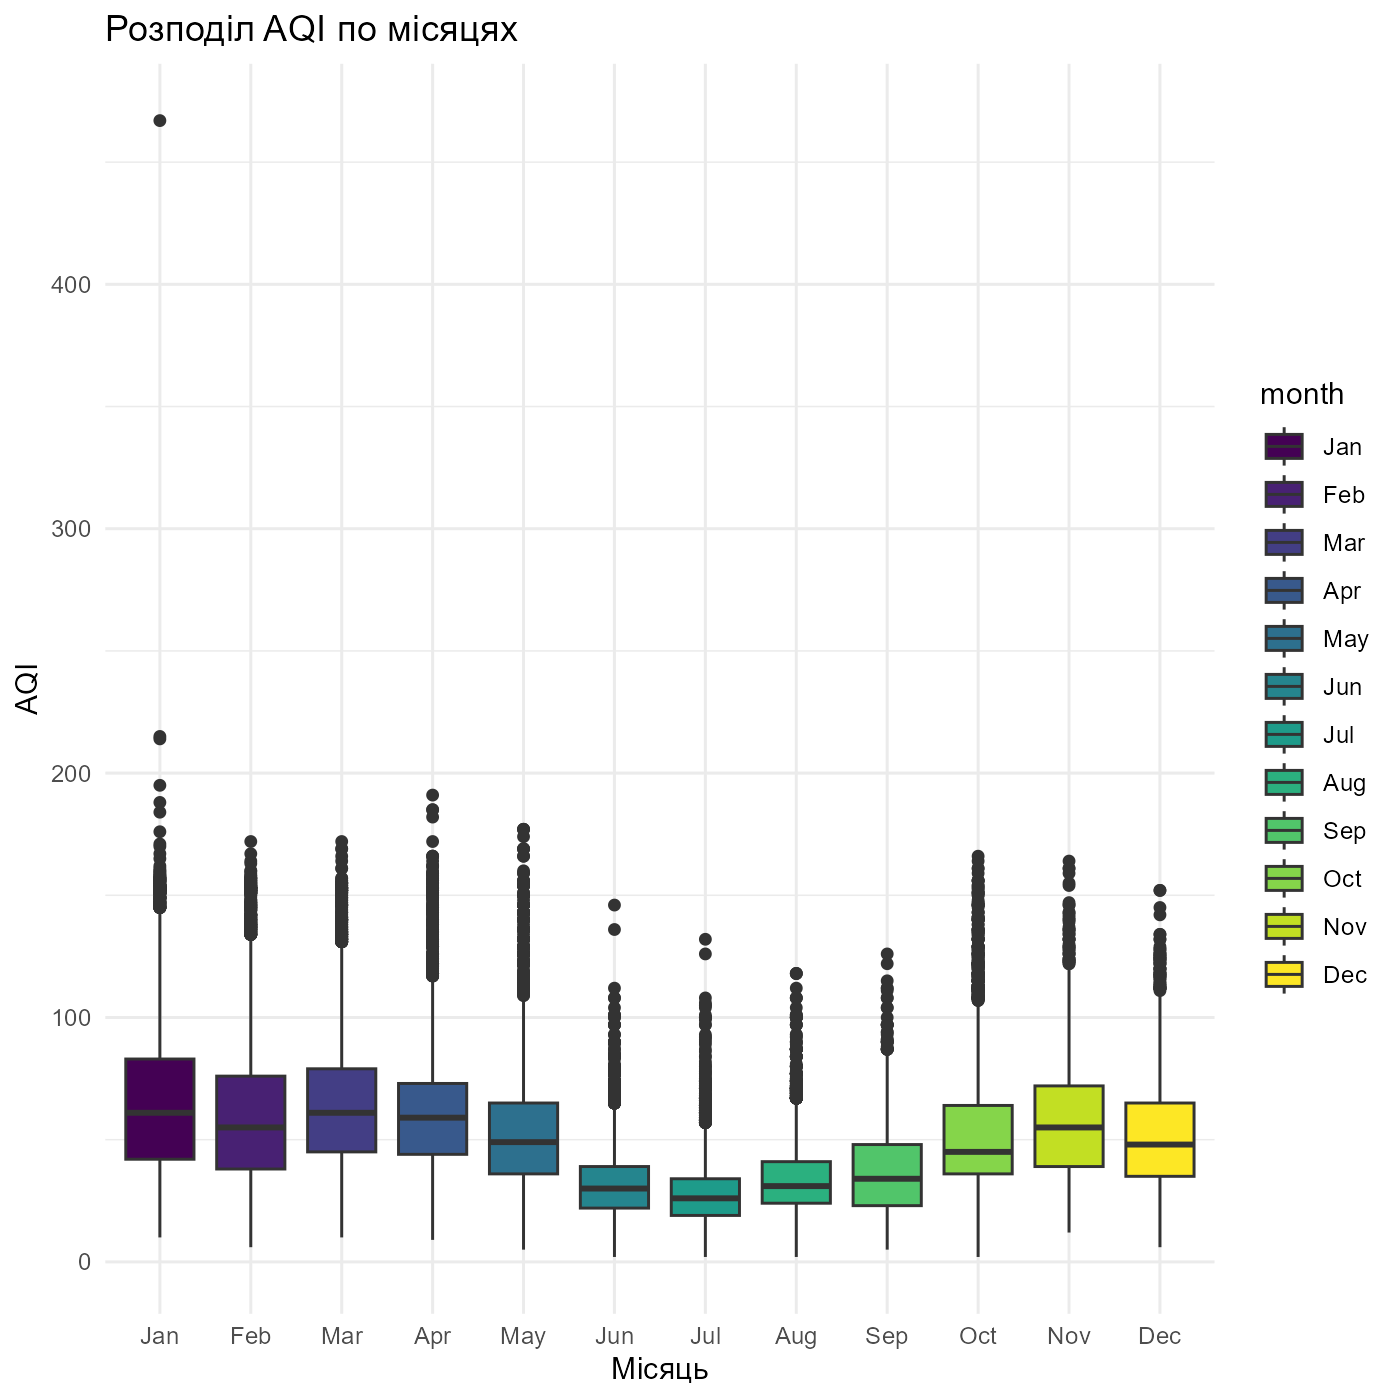
\includegraphics[width=2.2in]{./plots/question4/seasonal_change.png} &
      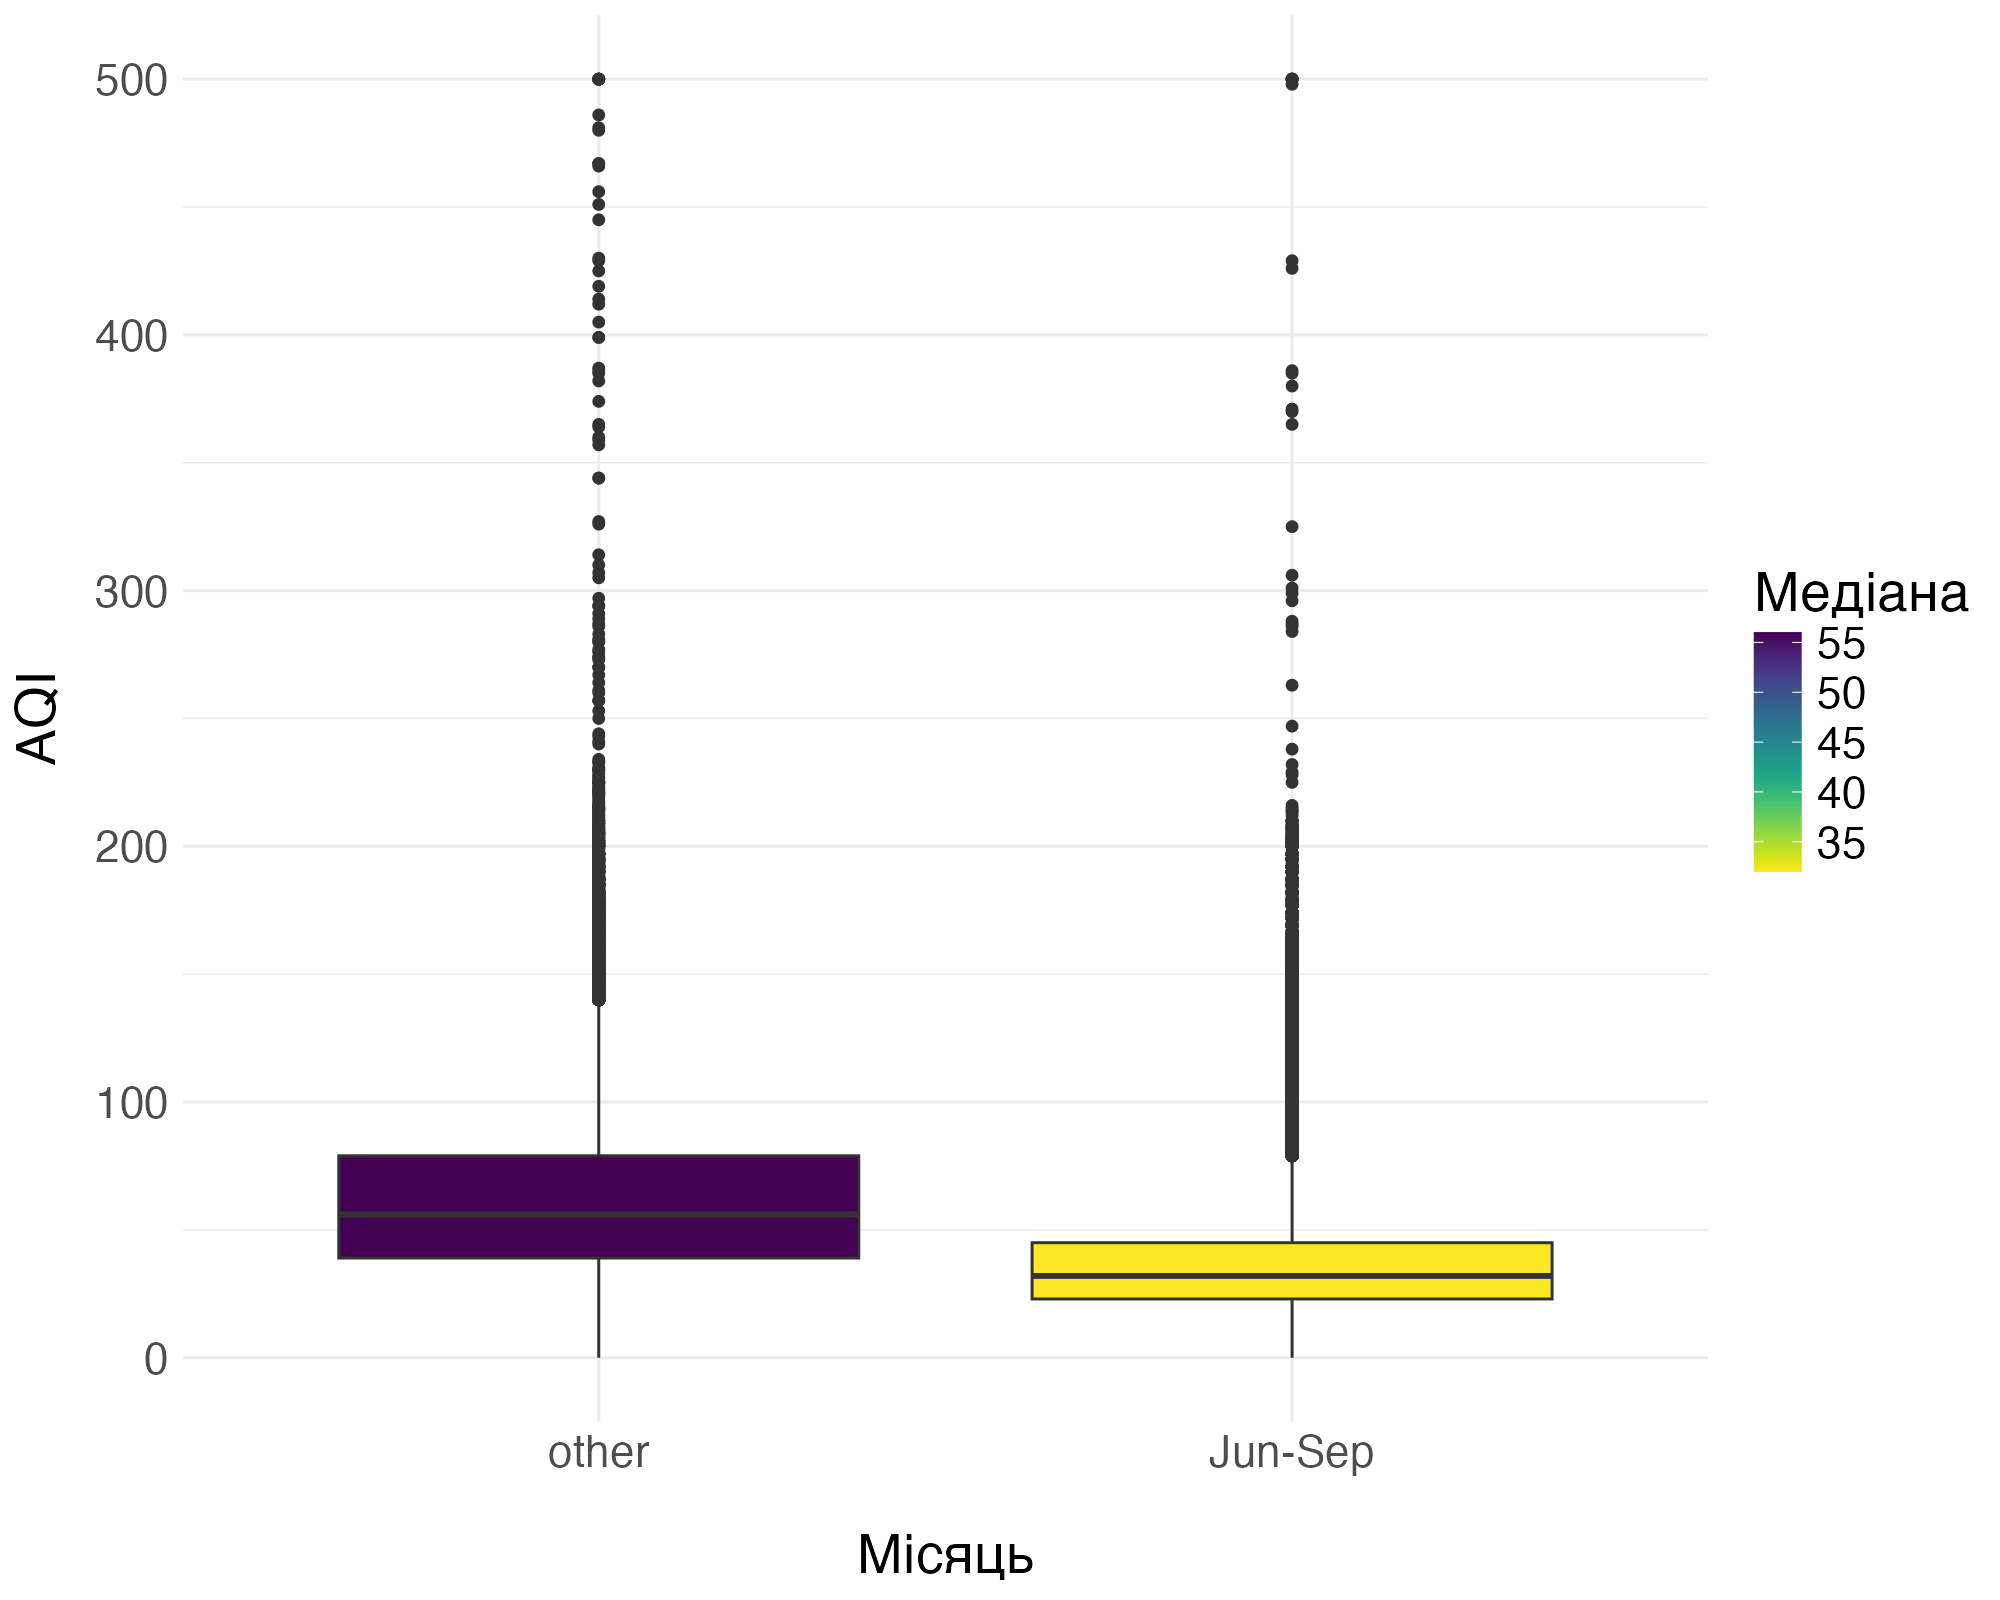
\includegraphics[width=2.2in]{./plots/lab2/hypotheses/season_vs_aqi.png}
    \end{tabular}
  \end{center}
\end{frame}

\begin{frame}
  \frametitle{Зменшення AQI влітку}

  \begin{enumerate}
    \item Розглянемо дві популяції:
    \begin{itemize}
      \item X - AQI від червня до вересня
      \item Y - AQI в інший час
    \end{itemize}
    
    \item Припустимо, що X і Y незалежні.  
    
    \item Нас цікавить різниця медіан $\theta = Me_X - Me_Y$.
    Їхніми оцінками $\hat{Me}_X$ і $\hat{Me}_Y$ будуть вибіркові медіани.  
  \end{enumerate}
\end{frame}

\begin{frame}
  \frametitle{Зменшення AQI влітку}

  \begin{enumerate}
    \item Обидві оцінки асимптотчно мають нормальний розподіл:
    $$\hat{Me}_i \overset{a}{\sim} N \bigg(\mu_i, \frac{1}{4n \cdot f(m)^2} \bigg); \quad i = X, Y$$
    де $n$ -- розмір вибірки, $f(x)$ -- щільність розподілу популяції, \linebreak $m$ -- медіана $f(x)$.   
  \end{enumerate}
  
\end{frame}

\begin{frame}
  \frametitle{Зменшення AQI влітку}

  \begin{enumerate}
    \item Оцінка різниці медіан $\hat{\theta} = \hat{Me}_X - \hat{Me}_Y$, теж асимптотично
    матиме нормальний розподіл, тому для тестування гіпотез можна використати тест Волда.  
    
    \item Проте, не знаючи $f(x)$, ми не зможемо порахувати дисперсію вибіркової медіани
    за наведеною формулою. Замість неї застосуємо бутстреп. Бутстреп-вибірки X* і Y* будуть
    генеруватися незалежно одна від одної, оскільки раніше ми припустили, що вони незалежні.  
  \end{enumerate}
\end{frame}

\begin{frame}
  \frametitle{Зменшення AQI влітку}

  \begin{enumerate}
    \item Маючи оцінку $\mathrm Var(\hat{\theta})$, перейдемо до тестування.  

    $H_0: \theta \ge 0$ vs. $H_1: \theta < 0$  
  
    $H_0: Me_X - Me_Y \ge 0$ vs. $H_1: Me_X - Me_Y < 0$

    \item Після обчислень отримуємо:
    
    $p = 7 \cdot 10^{-232}$

    Довiрчий iнтервал: $ (- \infty, -22.78492] $

    \item Отримали дуже низьке $p-value$ і довірчий інтервал, 
    який не включає нуль, тому відкидаємо гіпотезу $H_0$. 
    Різниця медіан є статистично значущою, і її значення, 
    на відміну від попереднього випадку, суттєве.
  \end{enumerate}
\end{frame}

\begin{frame}
  \frametitle{Вплив реформи на AQI}

  \begin{enumerate}
    \item Одним із головних питань EDA було, чи вплинула реформа на якість повітря. 
    \item Візуалізація розподілів AQI за періоди часу до 2017-05-25 (до введення реформи) і 
    після 2024-03-15 (найновіші дані) створює підстави для оптимізму.
  
    \begin{center}
      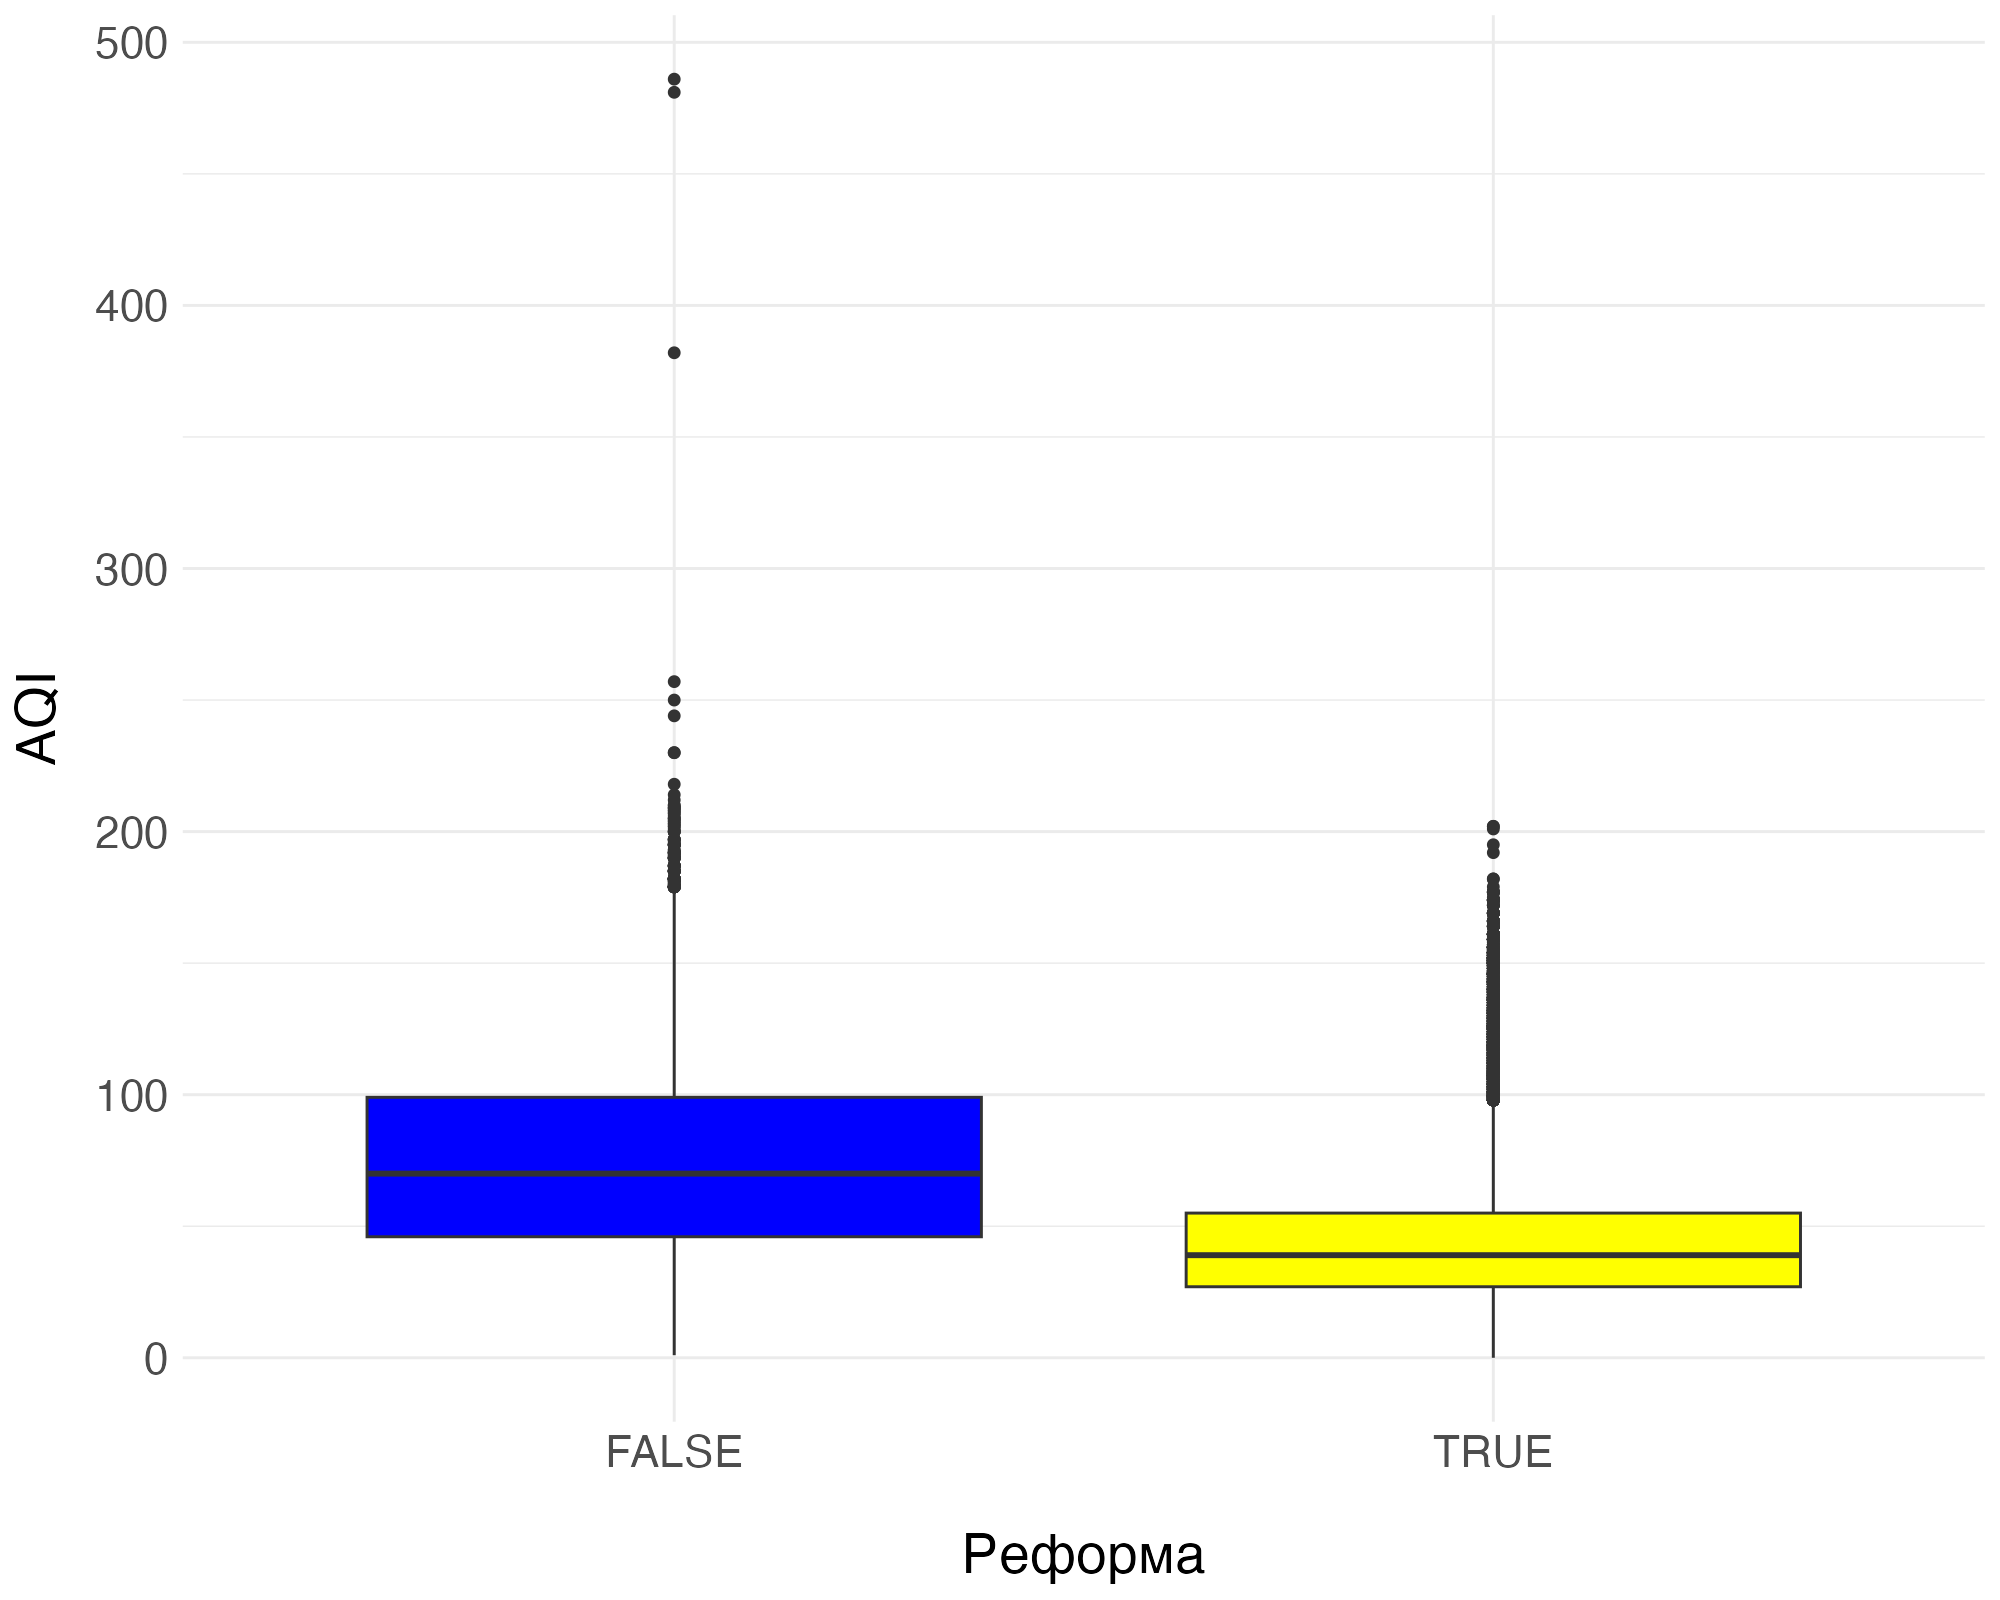
\includegraphics[height=1.8in]{./plots/lab2/hypotheses/reform_vs_aqi.png}
    \end{center}
  \end{enumerate}
\end{frame}

\begin{frame}
  \frametitle{Вплив реформи на AQI}

  \begin{enumerate}
    \item Розглянемо дві популяції:

    \begin{itemize}
      \item X - AQI до 2017-05-25
      \item Y - AQI після 2024-03-15
    \end{itemize}

    \item Аналогічно попередньому прикладу припустимо, що вони незалежні, 
    і будемо досліджувати різницю медіан $\theta = Me_X - Me_Y$.  
    
    \item Спочатку знайдемо $\mathrm Var(\hat{\theta})$ за допомогою бутстрепа.
  \end{enumerate}
\end{frame}

\begin{frame}
  \frametitle{Вплив реформи на AQI}

  \begin{enumerate}
    \item Протестуємо гіпотезу.  

    $H_0: \theta \le 0$ vs. $H_1: \theta > 0$  

    $H_0: Me_X - Me_Y \le 0$ vs. $H_1: Me_X - Me_Y > 0$
    
    \item Після обчислень отримуємо:
    
    $p = 8.26012 \cdot 10^{-256}$

    Довiрчий iнтервал: $ [30.4584230027386, \infty) $
  \end{enumerate}
\end{frame}

\begin{frame}
  \frametitle{Вплив на забруднювачі}

  Перевіримо гіпотезу, що введення реформи позитивно вплинуло на всі види забруднювачів.

  \begin{tabular}{lcccccc}
    \hline
    pollutant & mean\_before & mean\_after & delta     & p\_value     & p\_value\_BH & reject\_BH \\
    \hline
    so2       &  3.01784     &  1.10726    &  -1.91057 & 0            & 0            & True       \\
    co        &  0.45362     &  0.26408    &  -0.18954 & 0            & 0            & True       \\
    o3        & 33.25967     & 28.63565    &  -4.62402 & 0            & 0            & True       \\
    pm10      & 52.62785     & 25.39316    & -27.23468 & 0            & 0            & True       \\
    pm2.5     & 25.57816     & 12.49049    & -13.08766 & 0            & 0            & True       \\
    no2       & 15.69378     &  8.51227    &  -7.18151 & 0            & 0            & True       \\
    nox       & 20.29655     & 11.09376    &  -9.20278 & 0            & 0            & True       \\
    no        &  4.60706     &  2.54124    &  -2.06582 & 0            & 0            & True       \\
    \hline
  \end{tabular}
  
\end{frame}

\begin{frame}
  \frametitle{Вплив на забруднювачі}

  Для всіх забруднювачів $p-value$ близьке до нуля, тому можна з впевненістю сказати, що всі концентрації зменшились після реформи.
\end{frame}

\begin{frame}
  \frametitle{Ефективність у різних регіонах}

  Перевіримо гіпотезу, що введення реформи знизило aqi для всіх регіонів Тайваню.

  \begin{tabular}{lcccccc}
    \hline
    county & mean\_before & mean\_after & delta & p\_value & p\_value\_BH & reject\_BH \\
    \hline
    Hsinchu County    & 68.62315 & 45.02938 & -23.59376 & 0 & 0 & TRUE \\
    Taichung City     & 74.63010 & 42.40490 & -32.22519 & 0 & 0 & TRUE \\
    Hsinchu City      & 63.94682 & 41.37017 & -22.57664 & 0 & 0 & TRUE \\
    Miaoli County     & 66.38956 & 42.91476 & -23.47479 & 0 & 0 & TRUE \\
    Taoyuan City      & 64.54563 & 43.78240 & -20.76323 & 0 & 0 & TRUE \\
    Changhua County   & 80.26728 & 46.97687 & -33.29040 & 0 & 0 & TRUE \\
    Nantou County     & 93.54719 & 47.14222 & -46.40496 & 0 & 0 & TRUE \\
    Yunlin County     & 96.00076 & 45.37146 & -50.62929 & 0 & 0 & TRUE \\
    Chiayi County     & 87.57875 & 47.59077 & -39.98798 & 0 & 0 & TRUE \\
    Tainan City       & 94.27654 & 45.40709 & -48.86945 & 0 & 0 & TRUE \\
    New Taipei City   & 62.32621 & 45.24372 & -17.08248 & 0 & 0 & TRUE \\
    Pingtung County   & 83.46474 & 39.95991 & -43.50483 & 0 & 0 & TRUE \\
    \hline
  \end{tabular}
\end{frame}

\begin{frame}
  \frametitle{Ефективність у різних регіонах}

  \begin{tabular}{lcccccc}
    \hline
    county & mean\_before & mean\_after & delta & p\_value & p\_value\_BH & reject\_BH \\
    \hline
    Keelung City      & 56.53361 & 38.39945 & -18.13415 & 0 & 0 & TRUE \\
    Taipei City       & 58.32069 & 45.57595 & -12.74473 & 0 & 0 & TRUE \\
    Chiayi City       & 100.6705 & 45.60894 & -55.06163 & 0 & 0 & TRUE \\
    Yilan County      & 47.14808 & 35.15205 & -11.99603 & 0 & 0 & TRUE \\
    Kaohsiung City    & 99.27346 & 43.72133 & -55.55212 & 0 & 0 & TRUE \\
    Lienchiang County & 77.37931 & 53.07934 & -24.29996 & 0 & 0 & TRUE \\
    Penghu County     & 61.86655 & 40.62956 & -21.23699 & 0 & 0 & TRUE \\
    Taitung County    & 36.16457 & 27.49729 & -8.667281 & 0 & 0 & TRUE \\
    Kinmen County     & 96.21423 & 49.67600 & -46.53823 & 0 & 0 & TRUE \\
    Hualien County    & 46.79310 & 33.17739 & -13.61570 & $4 \cdot 10^{-297}$ & $4 \cdot 10^{-297}$ & TRUE \\
\end{tabular}
\end{frame}

% Висновки по ЛР2

\begin{frame}
  \section{Висновок}

  \frametitle{Зміст}
  \tableofcontents[currentsection]
\end{frame}

\begin{frame}
  \frametitle{Узагальнений висновок}
  Статичтичні методи, які були використані в цій лабораторній роботі, 
  дозволяють грунтовно оцінити якість тих чи інших показників якости повітря у регіонах Тайваню.
  
\end{frame}

\end{document}